\documentclass[article]{jss}

%% -- LaTeX packages and custom commands ---------------------------------------
%% my packages
\usepackage{graphicx} % table rotate
\usepackage{array} %table height
\usepackage{pdfpages} %include pdf
\usepackage{amsmath} %math equation
\usepackage{amssymb} %math (real number symbol)
\usepackage[utf8]{inputenc} %debug for in not ASCII
%\usepackage[]{algorithm2e} % for pseudo code
\usepackage{float} % figure H
\usepackage{subfig}
\usepackage{enumerate} %i ii iii.....
\usepackage{listings} %for code chrunk
\usepackage{ctable} % for \specialrule command

%\usepackage{svg}

%% recommended packages
\usepackage{thumbpdf,lmodern}

%% another package (only for this demo article)
\usepackage{framed}
\usepackage{float} %for figure [H]
%% new custom commands
\newcommand{\class}[1]{`\code{#1}'}
\newcommand{\fct}[1]{\code{#1()}}
\newcommand{\imgdir}{../../../paperImage/}
%% For Sweave-based articles about R packages:
%% need no \usepackage{Sweave}
%\SweaveOpts{engine=R, eps=FALSE, keep.source = TRUE}


%% -- Article metainformation (author, title, ...) -----------------------------

%% - \author{} with primary affiliation
%% - \Plainauthor{} without affiliations
%% - Separate authors by \And or \AND (in \author) or by comma (in \Plainauthor).
%% - \AND starts a new line, \And does not.
\author{Bo-Syue Jiang\\National Taipei University
\And Han-Ming Wu\\National Chengchi University}
\Plainauthor{Bo-Syue Jiang,Han-Ming Wu}

%% - \title{} in title case
%% - \Plaintitle{} without LaTeX markup (if any)
%% - \Shorttitle{} with LaTeX markup (if any), used as running title
\title{ggESDA: An \proglang{R} Package for Exploratory Symbolic Data Analysis using \pkg{ggplot2}}
\Plaintitle{ggESDA: An R Package for Exploratory Symbolic Data Analysis using ggplot2}
\Shorttitle{ggESDA package in R}

%% - \Abstract{} almost as usual
\Abstract{
  This paper presents the \pkg{ggESDA} package, which we developed for exploratory symbolic data analysis in \proglang{R}. Based on \pkg{ggplot2} \cite{Wickham:2009}, the \pkg{ggESDA} package which is familiar programming structure with its parent provides a wide variety of graphical techniques such as histogram, 3D-scatterplot and radar plot. In addition, a general and  customized transformation function \code{classic2sym} is implemented for generating a symbolic data table from classical data frame by clustering algorithm, \pkg{RSDA} \cite{Rojas:2015} function and user-defined method. wait for edit......
}

%% - \Keywords{} with LaTeX markup, at least one required
%% - \Plainkeywords{} without LaTeX markup (if necessary)
%% - Should be comma-separated and in sentence case.
\Keywords{data visualization, symbolic data analysis, exploratory data analysis, \pkg{ggplot2} extensions, interval-valued data, \proglang{R}}
\Plainkeywords{data visualization, symbolic data analysis, exploratory data analysis, ggplot2 extensions, interval-valued data, R}

%% - \Address{} of at least one author
%% - May contain multiple affiliations for each author
%%   (in extra lines, separated by \emph{and}\\).
%% - May contain multiple authors for the same affiliation
%%   (in the same first line, separated by comma).




\begin{document}
%\SweaveOpts{concordance=TRUE} 
\section{Introduction}
"In Data Science the aim is to extract new knowledge from Standard, Big, and complex data. Often these data are unstructured with variables defined on different kinds of units. They can also be multi-sources (as mixtures of numerical and textual data, with images and networks)." \cite{Diday:2018}. The statement indicates that not only conventional data but the unstructured data, also known as symbolic data, is vital for data science. Rather than the classical data represented by a single value, symbolic data with measurements on $p$ random variables can be $p$-dimensional statistical units such as hypercubes or histograms. The field of symbolic data analysis (SDA) \cite{Billard+Diday:2007} is to broaden the application aspects of statistical methodologies, extend traditional cognition of a form of data unit and build a brand-new analysis system of data science. Recent developments in the field of big data analytics have led to a renewed interest in complex structure data such as symbolic data. As shown in Figure \ref{fig:trend}, the number of researches in SDA represents an increasing trend from 1998 to 2020, which outstands the importance of it during the years.



\begin{figure}[htbp]	
  		\centering	 			 	 
 	 		%\includegraphics[width=1\textwidth]{\imgdir Trend_SDA_1998_to_2020.png} 
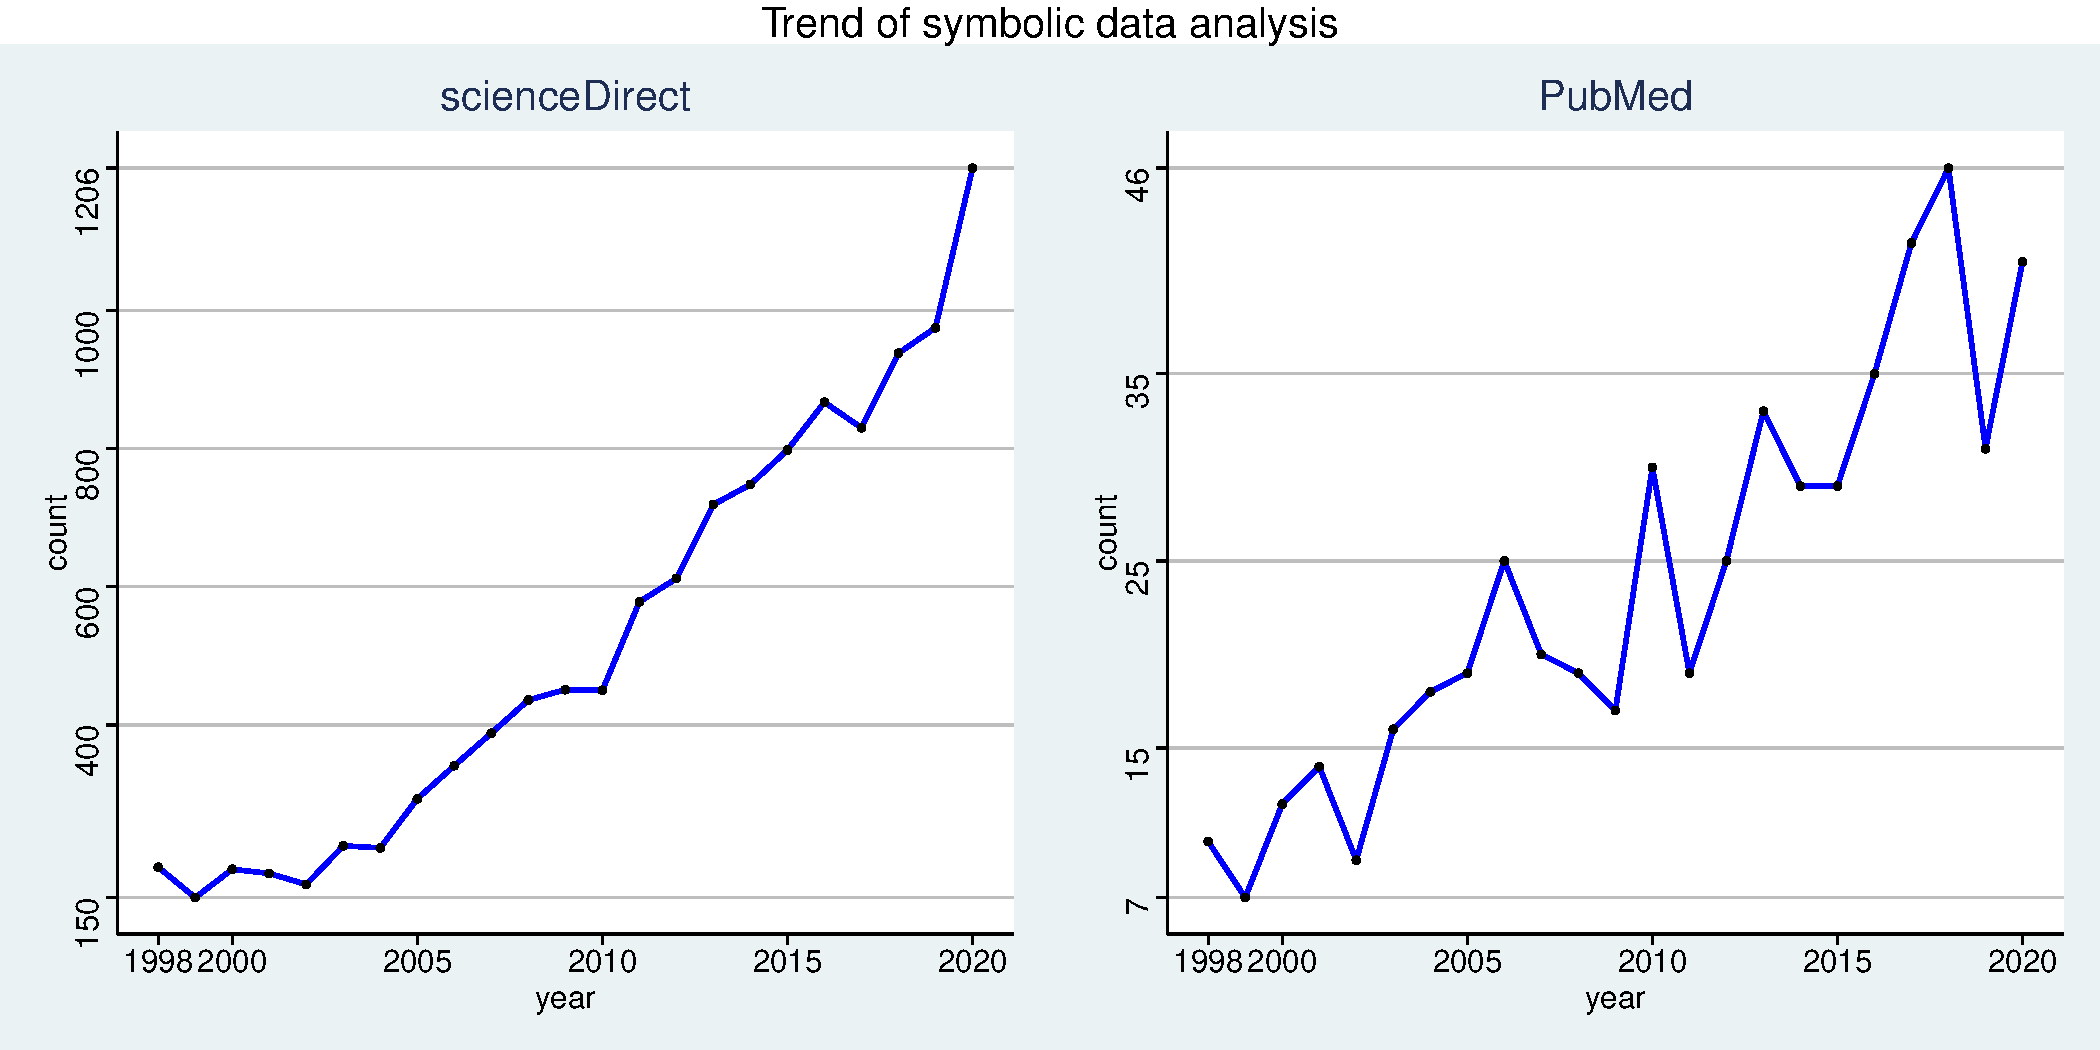
\includegraphics{ggESDA_Jiang&Wu_20210915-TrendFig}
  		\caption{The number of "symbolic data analysis" or "interval-valued data" related articles in researches and applications according to PubMed and ScienceDirect online database over time from 1998 to 2020.}   		
  		\label{fig:trend}   			 		 
\end{figure}

Among ScienceDirect, Engineering and Computer Science lead the subject areas obviously, shown in Figure \ref{fig:subjectAreas}.

\begin{figure}[htbp]	
  		\centering	 			 	 
 	 		%\includegraphics[width=1\textwidth]{\imgdir subjectAreas_scienceDirect.png} 
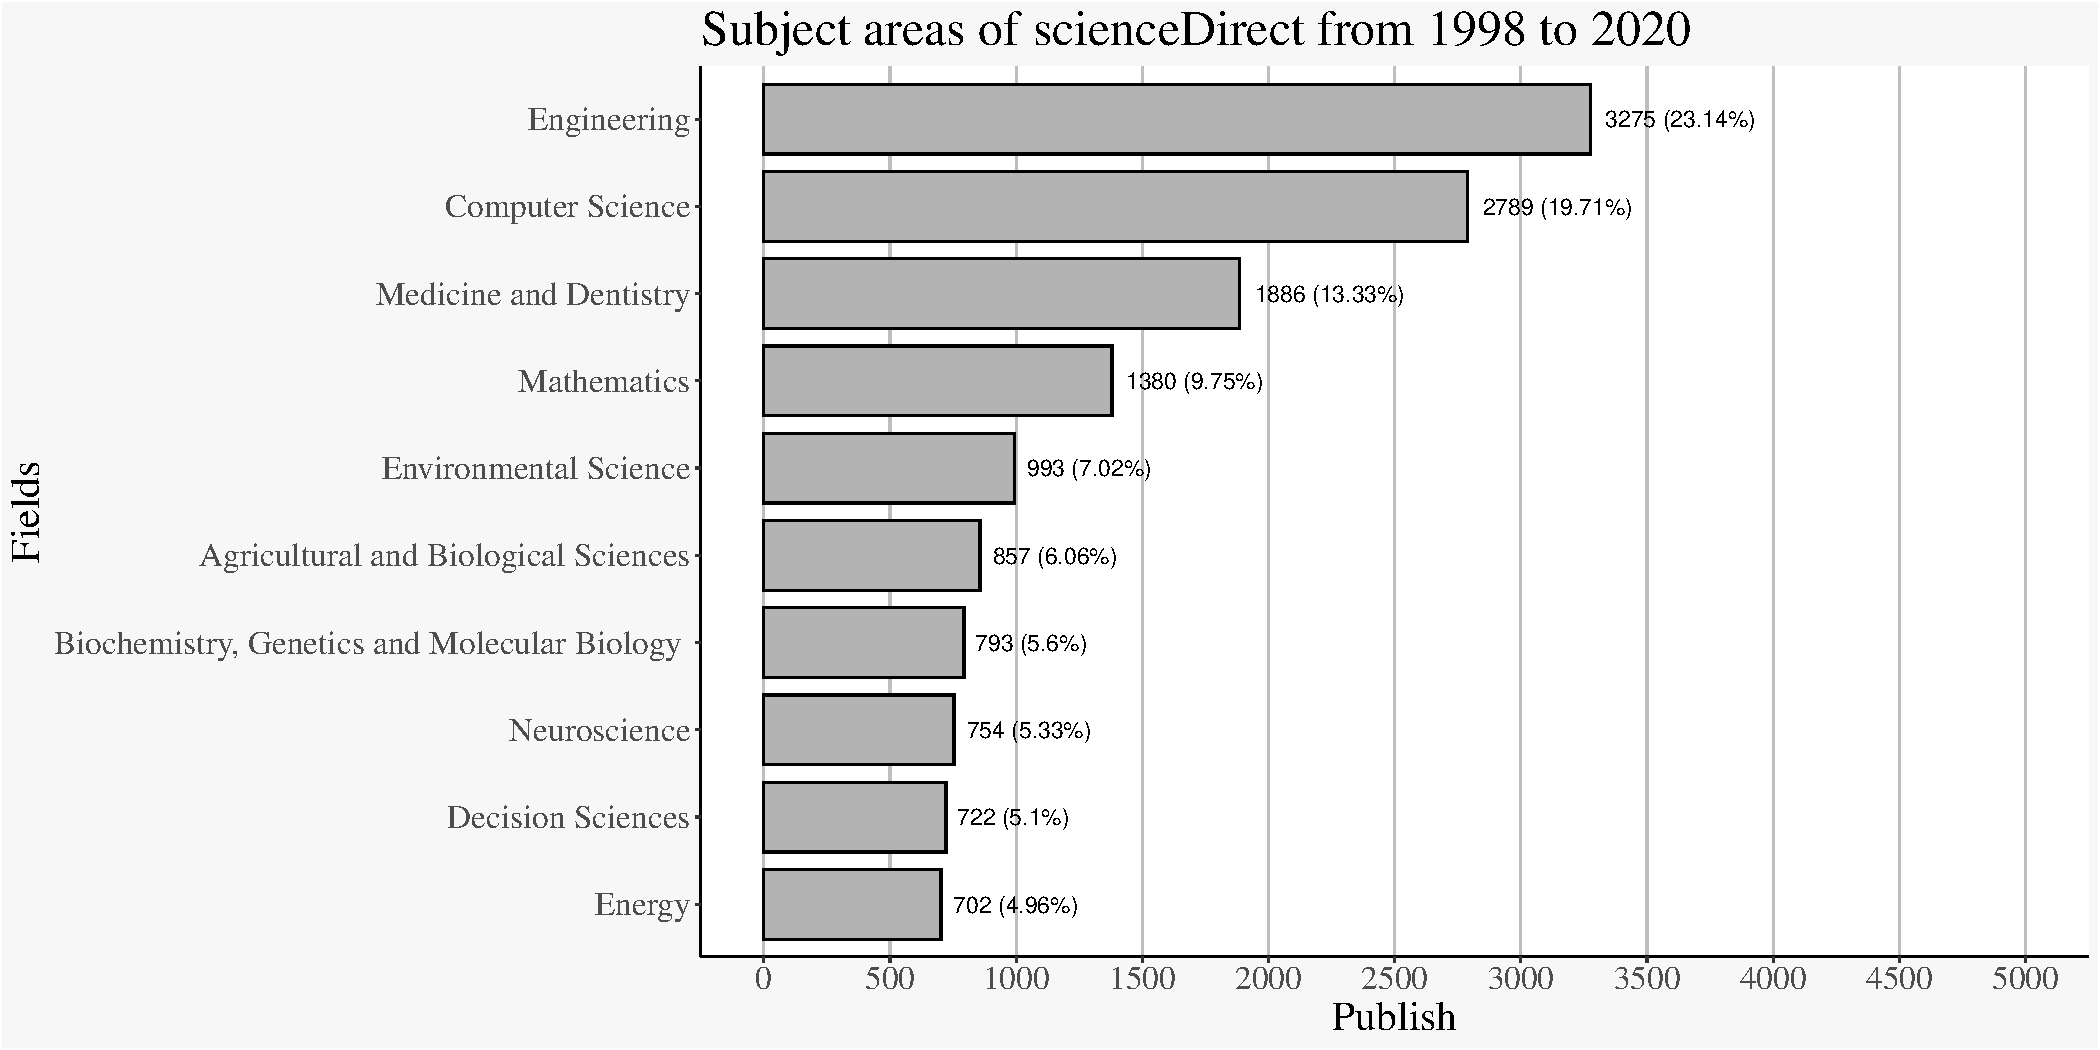
\includegraphics{ggESDA_Jiang&Wu_20210915-subjectFig}
  		\caption{Top 10 researches and applications domains for SDA or interval-valued data (ScienceDirect) from 1998 to 2020} 
  		\label{fig:subjectAreas}   			 		 
\end{figure}


In practice, the symbolic data is often generated by aggregating massive datasets into intervals in order to make the management easy and appropriate. An interval-valued symbolic random variable $X$, taking values in interval, can be denoted such as $X = [a,b] \subset  R^{1}$, where $a \leq b$, and $a, b \in R^{1}$. Let the random variable $X$, for instance, be the weight, then $X = [50,100]$ represents the interval covering the weight of people. With the advent of big data analytic, interval-valued data is becoming more common and accessible than ever. The researches for interval-valued data such as the sign test for COVID-19 data \cite{sherwani:2021}, the prediction via regularized artificial neural network \cite{yang:2019}, a bivariate Bayesian method for regression models \cite{xu:2021}, etc.

Exploratory Data Analysis (EDA) \cite{Tukey:1977} is primarily used to see what data can reveal beyond the formal modeling or hypothesis testing task, provides an overview of raw datasets and obtains a general understanding about the variables and their relationships.

%end introduction

\section{why SDA plot (weakness of classical plot)}

\subsection{sol overstike}
For the conventional exploratory data analysis, it is always a severe challenge to deal with enormous datasets because conventional displays suffered from overstrikes of data points representing the value (scatterplot type displays) or overstrikes of line segments connecting values of neighboring variables. As a consequence, exploratory symbolic data analysis (SDA) becomes a preliminary yet essential tool for summarizing the main characteristics of a data set before appropriate statistical modeling can be applied. Besides escaping the problem mentioned above, SDA can effectively reduce observations in data, which will make the study focus on what we interesting instead of unnecessary information such as Figure~\ref{fig:compare}.

\begin{figure}[htbp]
\centering
\scalebox{0.8}{
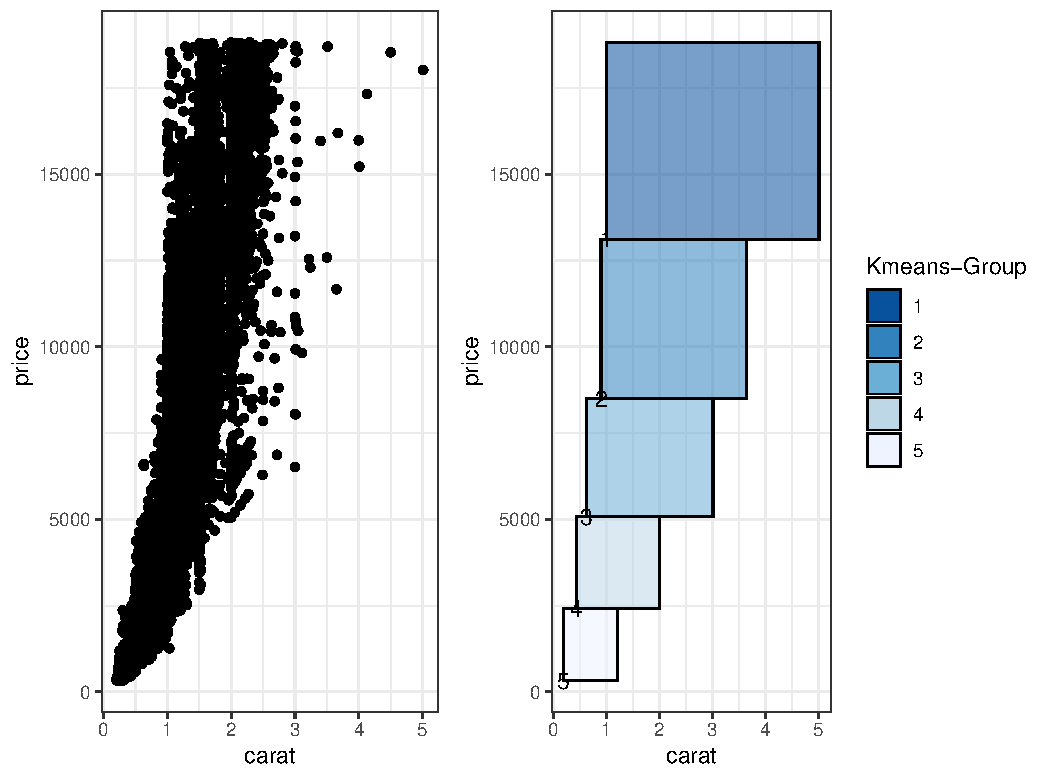
\includegraphics{ggESDA_Jiang&Wu_20210915-compare}
}
\caption{\label{fig:compare} Compare classical data and symbolic data}
\end{figure}

In Figure~\ref{fig:compare}, we can clearly visualize the scatter plot in the right hands, which is represented by symbolic data and aggregated by K-means \cite{macqueen:1967}. 


\subsection{full information}

In the past, we would like to use barplot to visualize the frequency of categorical data, but that was merely represented the distribution of full data in that category. It cannot lead researchers to explore more details in what they are interesting such as a particular part of data, so aggregation methods play a vital role to merge the data we interesting.

However, the conventional categorical data after merging will usually be represented by mode, which will be unmeaningful to visualize and cause the loss of information that may become larger when the data or the number of factors in that category is growing on. SDA will build a histogram by calculating each factor of the category of frequency as bins to solve this kind of problem as a result. In that way, a categorical variable will never be shown as a single value at all, instead, a complete information histogram will be substituted.



\subection{Prominent SDA Packages}

The most prominent packages on CRAN are commonly used for statistical or machine learning analyze. It can be briefly classified into two parts, one is focused on statistic analysis, and the other is general SDA packages including both analysis method and some graphical technology. Nevertheless, most of their graphical technology tends to use the basic graphics in \proglang{R} rather than \pkg{ggplot2}, or only visualizes univariate distribution which is difficult to present the relationship between variables. 

On the contrary, \pkg{ggESDA} uses a high-level graphic system by \pkg{ggplot2} to solve the problem mentioned above and provides a variety of EDA methods in all kinds of the variate, which can be summarized as the table \ref{tab:pkgCompare}. The number in table \ref{tab:pkgCompare} shows how many methods are provided in its field.

%begin : this is my table for package_compare 
%\begin{table}[htbp]
\begin{table}[h]
  \centering
  \caption{Compare with \proglang{R} packages}
  %\rotatebox[origin=c]{90}{
  \setlength{\extrarowheight}{6pt}
  \resizebox{\textwidth}{!}{
    \begin{tabular}{|l|l|c|c|ccc|c|c|c|}
    
    \toprule
    \multicolumn{1}{r}{} & \multicolumn{1}{r}{} & \multicolumn{1}{c}{\textbf{ Available}} & \multicolumn{1}{c}{\textbf{Summarize}} & \multicolumn{3}{c}{\textbf{EDA}} & \multicolumn{1}{c}{\textbf{Statistic}} & \multicolumn{2}{c}{\textbf{Machine learning}} \\\hline
    \multicolumn{1}{c|}{Package} & \multicolumn{1}{c|}{Author} & Version & Function & Univariate & Bivariate & Multivariate & Stat. Method & Supervised & \multicolumn{1}{c}{Unsupervised} \\\hline
    RSDA  & Rojas et al. (2015) & R(4.1.0)     & \code{classic.to.sym}     & -     & 1     & -     & 3     & \textbf{2}    & \textbf{1} \\
    symbolicDA & Dudek et al. (2013) & R(4.1.0)     &    -   & -     & -     & \textbf{2}    & 2     & 1     & \textbf{1} \\
    HistDAWass & Irpino (2015) & R(4.1.0)     & \code{data2hist}     & 4     & -     & -     & 3     & 1     & \textbf{1} \\
    
    MAINT.Data & Silva \&  Brito (2011) & R(4.1.0)     &   -    & -     & -     & -     & \textbf{7}    & -     & \textbf{1} \\\hline
    iRegression & Neto et al. (2011) & R(4.1.0)     &   -    & -     & -     & -     & 1     & -     & - \\
    intReg & Toomet (2012) & R(3.6.0)      &  -     & -     & -     & -     & 1     & -     & - \\
    ISDA.R & Filho \&  Fagundes (2012) & R(2.15.2)      &    -   & 1     & -     & 1     & 1     & -     & - \\
    GPCSIV & Brahim (2013) & R(3.0.2)      &  -     & -    & -     & -     & 1     & -     & - \\
    GraphPCA & Brahim \& Kallyth (2014) & R(4.1.0)      &   -    & -     & 1     & 1     & 1     & -     & - \\
    \midrule
    ggESDA & Jiang (2021) & R(4.1.0)     & \code{classic2sym}     & \textbf{8}    & \textbf{4}    & \textbf{2}    & 1     & -     & - \\
    \bottomrule
    \end{tabular}}%
  \label{tab:pkgCompare}%
\end{table}%
%end : this is my table for package_compare 

In \proglang{python}, we can also find the SDA package such as \pkg{iardacil} \cite{umbleja:2020} which is available from the Github at \url{https://github.com/iardacil/SDA}. The zoomstart software in \pkg{iardacil} is provided with SODAS software project \cite{diday:2008}. It is a basic thinking for general radar plot, improved for distinct groups visualization by \pkg{ggESDA}, and implemented in \proglang{R} using \pkg{ggplot2}.



%end why ggESDA

\section{Basic numerical summaries}

The main content of EDA relates to the basic numerical summaries of data (e.g., the central tendency measures, and variation or variability measures) and the basic graphical summaries of data. For example, the five-number summary of numerical data (minimum, $25\%$ quartiles, median, $70\%$ quartiles, and maximum) is used to construct a boxplot. In the field of SDA, there are many algorithms to calculate descriptive statistics and frequency for interval-valued data, and we will illustrate the univariate and bivariate summaries respectively.

\subsection{Univariate summaries}

To build a statistic chart or analysis, descriptive statistics are necessary to be constructed, as well as the frequency occurring in each bin in a histogram chart. For a histogram chart, subdivisions of it into equidistant and non-equidistant will also be consider in this section.

\subsubsection{Descriptive statistics}

For the quantile in interval-valued data, summarizing it may seem to be obvious to separate data into a minimum and maximum data table, then calculate quantiles of both data tables to build a new interval-valued quantile data table.

In statistics, it may be more interesting to discuss mean and variance in a particular random variable $Z$; see \cite{bertrand:2000}. The realization of $Z$ for the observation $W_u$ is the interval $Z(W_u) = [a_u,b_u]$, where $u=1,2,\cdots,m$ and $m$ is the number of concepts.

First of all, assume that each object is equally likely to be observed with probability $\frac{1}{m}$, and the empirical density function of $Z$ is defined as : 

\begin{equation}\label{eq:dist1}
f(\xi) = \frac{1}{m} \sum_{u:\xi \in Z(W_u)}(\frac{1}{b_u-a_u})
\end{equation}

where $\xi$ is the individual descriptions.


The Equation (\ref{eq:dist1}) is also equivalently to :

\begin{equation}\label{eq:dist2}
f(\xi) = \frac{1}{m}\sum_{u \in E}\frac{I_u(\xi)}{\| Z(u) \|}\;,\xi \in \mathbb{R}
\end{equation}

where $I_u(.)$ is the indicator function that $\xi$ is or is not in the interval $Z(u)$, $\| Z(u) \|$ is the length of that interval, and $E=\{w_1,w_2,\cdots,w_m \}$.

Further, the symbolic sample mean from definition for $Z$ is $\bar{Z} = \int_{-\infty}^{\infty} \xi f(\xi)\;d\xi$, which can be reduced as :

\begin{equation}\label{eq:mean}
\bar{Z}=\frac{1}{m}\sum_{u \in E}\frac{a_u+b_u}{2}
\end{equation}

Finally, after getting the sample mean, the symbolic sample variance can be defined as follow:

\begin{equation}\label{eq:varDef}
\begin{split}
S^2 & = \int_{-\infty}^{\infty} (\xi - \bar{z})^2f(\xi)\;d\xi \\
 & = \int_{-\infty}^{\infty} \xi^2f(\xi)\;d\xi-\bar{z}
\end{split}
\end{equation}

and substituting for $f(\xi)$ from Equation (\ref{eq:dist2}), we have 
\begin{equation}\label{eq:derived}
\begin{split}
\int_{-\infty}^{\infty} \xi^2f(\xi)\;d\xi &= \frac{1}{m}\sum_{u \in E}\int_{-\infty}^{\infty} \xi^2 \frac{I_u(\xi)}{\| Z(u) \|}\;d\xi \\
&= \frac{1}{m}\sum_{u \in E} \int_{a_u}^{b_u} \frac{\xi^2}{(b_u-a_u)}\;d\xi \\
&= \frac{1}{3m} \sum_{u \in E}(\frac{b_u^3 - a_u^3}{b_u-a_u})
\end{split}
\end{equation}

Hence,
\begin{equation}\label{eq:var}
S^2 = \frac{1}{3m} \sum_{u \in E}(a_u^2+a_ub_u+b_u^2)-\frac{1}{4m^2}\left[ \sum_{u \in E}(a_u+b_u) \right]^2
\end{equation}

\subsubsection{Histogram Frequency}\label{sec:hist}

For the univariate histogram frequency, assume that we partition the interval $I=[\min_{u \in E} a_u,\\ \max_{u \in E} b_u]$ into $r$ subintervals, and all of them in the histogram are equal distance. That is, $I_g = [\zeta_{g-1},\zeta_{g}),g=1,2,\cdots,r$, then $\| I_j \| = \| I_k \| , j,k=1,2,\cdots,r$. As a consequence, the observed frequency of the interval-valued variate $Z$ for the histogram subinterval $I_g$ from the definitions is

\begin{equation}\label{eq:fg}
f_g = \sum_{u \in E}\frac{\| Z(u) \cap I_g \|}{\| Z(u) \|}
\end{equation}

Moreover, for the interval-valued variate $Z$, we can pool the $a_u$ and $b_u$ from the interval of all observations, and sort it as a new vector $(x^{(1)},x^{(2)},\ctors,x^{(2m)})$ to represent the cut of a histogram. The subinterval from the cut is then defined as $I'_g = [x^{(j)},x^{(j+1)})$, where $j = 1,2,\cdots, 2m-1$, and apply the Equation (\ref{eq:fg}) to get frequency. In most cases, $\| I'_g \|$ will not be equal to another, so we can get another histogram type, called non-equidistant-bin histogram.


\subsection{Bivariate summaries}

Many of the principles developed for the univariate case can be expanded to a general $p$-variate case, $p > 1$. We shall focus attention on obtaining joint histograms for $p = 2$. The following will reveal the statistics and bivariate histogram.

\subsubsection{Descriptive statistics}

For bivariates interval-valued variables, $Z_1$ and $Z_2$, the observations $u$, where $u \in E$, on the rectangle $Z(u) = Z_1(u) \times Z_2(u)$ is $([a_{1u}, b_{1u}], [a_{2u}, b_{2u}])$. Assume the individual description vectors $\xi$ are each uniformly distributed over the respective intervals $Z_1(u)$ and $Z_2(u)$.  Define the empirical joint density function for $(Z_1, Z_2)$:

\begin{equation}\label{eq:bi_density}
f(\xi_1,\xi_2)=\frac{1}{m}\sum_{u \in E}\frac{I_u(\xi_1,\xi_2)}{\| Z(u) \|}
\end{equation}

where $I_u(\xi_1,\xi_2)$ is the indicator function that $(\xi_1,\xi_2)$ is or is not in the rectangle $Z_u$ and where $\|Z(u)\|$ is the area of this rectangle.

There is three methods to calculate bivariate interval-valued variables covariance function. For the first one, it can be derived by \cite{billard:2003} as following:

\begin{equation}\label{eq:cov}
cov(Z_1,Z_2)=\frac{1}{4m}\sum_{u \in E}(b_{1u} + a_{1u})(b_{2u} + a_{2u})-\frac{1}{4m^2}\left[ \sum_{u \in E}(b_{1u} + a_{1u}) \right]\left[ \sum_{u \in E}(b_{2u} + a_{2u}) \right]
\end{equation}

Second, an alternative expression of the symbolic sample variance for $Z$ in Equation (\ref{eq:var}) can be expressed as

\[
S^2 = \frac{1}{3m}\sum_{u \in E}\left[  (a_u-\bar{Z})^2 +(a_u-\bar{Z})(b_u-\bar{Z})+(b_u-\bar{Z})^2 \right]
\]

The above equation can be generalized by \cite{Billard+Diday:2007} to formulate the form of the symbolic sample covariance for $Z_j$ and $Z_{j\prime}$ as

\begin{equation}\label{eq:gq_cov}
cov(Z_j,Z_{j^{ \prime}}) = \frac{1}{3m}\sum_{i=1}^{m}G_jG_{j^{\prime}}\left[ Q_jQ_{j^\prime} \right]^{1/2}, \;\;j,j^\prime=1,2,\cdots,p
\end{equation}

where for $J = j,j^\prime$, 

\[
\begin{split}
Q_J &= (a_{iJ} - \bar{Z_J})^2 +(a_{iJ} - \bar{Z_J})(b_{iJ} - \bar{Z_J})+(b_{iJ} - \bar{Z_J})^2,\\
G_J &= \left\{\begin{array}{l}
          \begin{split}
          -1 &, \;\;\mbox{if} \;\; \xi_{iJ}^{c} \leq \bar{Z_J}\\
           1 &,  \;\;\mbox{if} \;\;  \xi_{iJ}^{c} > \bar{Z_J}
           \end{split}
        \end{array}\right.
\end{split}
\]

and $\xi_{iJ}^{c}$ is the midpoint of the interval $[a_{iJ},b_{iJ}]$.

Last, it was further demonstrated by \cite{billard:2007} and \cite{billard:2008} that the sample variance in Equation (\ref{eq:var})
is a function of the total sum of squares (SST) and that the SST can be decomposed into the sum of the internal (within) variation and the between variation. The total sum of products (SPT) is the sum of the within sum of products and the between sum of products. The Equation (\ref{eq:var}) was also extended to the bivariate case to obtain the sample covariance of $Z_j$ and $Z_{j^\prime}$ based on the decomposition of the SPT as

\begin{equation}\label{eq:spt_cov}
\begin{split}
cov(Z_j,Z_{j^{ \prime}}) = \frac{1}{6m}\sum_{i = 1}^m \left[ 2(a_{ij}-\bar{Z}_j)(a_{ij^\prime}-\bar{Z}_{j^\prime}) +(a_{ij}-\bar{Z}_j)(b_{ij^\prime}-\bar{Z}_{j^\prime})\\
+(b_{ij}-\bar{Z}_j)(a_{ij^\prime}-\bar{Z}_{j^\prime})+2(b_{ij}-\bar{Z}_j)(b_{ij^\prime}-\bar{Z}_{j^\prime})\right]
\end{split}
\end{equation}

The definitions and calculations of the symbolic sample covariance in
Equations (\ref{eq:cov})-(\ref{eq:spt_cov}) are consistent with the results in the classic data case if $a_{ij}=b_{ij}$ for $i = 1,2,\cdots,m ,\; j = 1,2,\cdots, p$. If $j = j^\prime$, the Equation (\ref{eq:spt_cov}) reduces to the sample variance of the interval-valued variable as given in Equation (\ref{eq:var}).


\subsubsection{2D-Histogram} \label{sec:hist2d}

Analogously with Equation (\ref{eq:fg}), we can find the joint histogram
for $(Z_1, Z_2)$ by graphically plotting $\{R_{g_1g_2},p_{g_1g_2}\}$ over the rectangles $R_{g_1g_2} = \{[\zeta_{1,g_1-1},\zeta_{1,g_1}) \times [\zeta_{2,g_2-1},\zeta_{2,g_2}) \},\; g_1 = 1,2,\cdots,r_1, \;g_2=1,2,\cdots,r_2$, where

\begin{equation}\label{eq:bi_fg}
f_{g_1g_2} = \sum_{u \in E}\frac{\| Z(u) \cap R_{g_1g_2} \|}{\| Z(u) \|}
\end{equation}

i.e., $f_{g_1g_2}$ is the number of observations that fall in the rectangle $R_{g_1g_2}$ and is not necessarily an integer value (except in the special case of classical data). The relative frequency that an arbitrary individual description vector lies in the rectangle $R_{g_1g_2}$ is therefore

\begin{equation}\label{eq:bi_rel_fg}
p_{g_1g_2} = \frac{f_{g_1g_2}}{m}
\end{equation}

%end basic numeric summarize


\section[The ggESDA package]{The \pkg{ggESDA} package}

\pkg{ggESDA} is now available from the Github at \url{https://github.com/kiangkiangkiang/ggESDA}. All reference manual documented by exported functions and introduction vignettes can also be download here. In the following section, we are going to illustrate the functionalities and syntaxes about \pkg{ggESDA}.
 
\subsection{General design}

The \pkg{ggESDA} object is composed of the interval-valued data, statistics data frame, clustering results, and other components from \pkg{R6} class. Based on it, the developed graphical technology can extend three aspects by its variables, univariate, bivariate, and multivariate. The \pkg{ggESDA} aims to convert the traditional data into the \pkg{ggESDA} object and visualizes the symbolic data using \pkg{ggplot2}, which is shown in Figure \ref{fig:pkgStr}.

\begin{figure}[h]	
  		\centering	 			 	
 	 		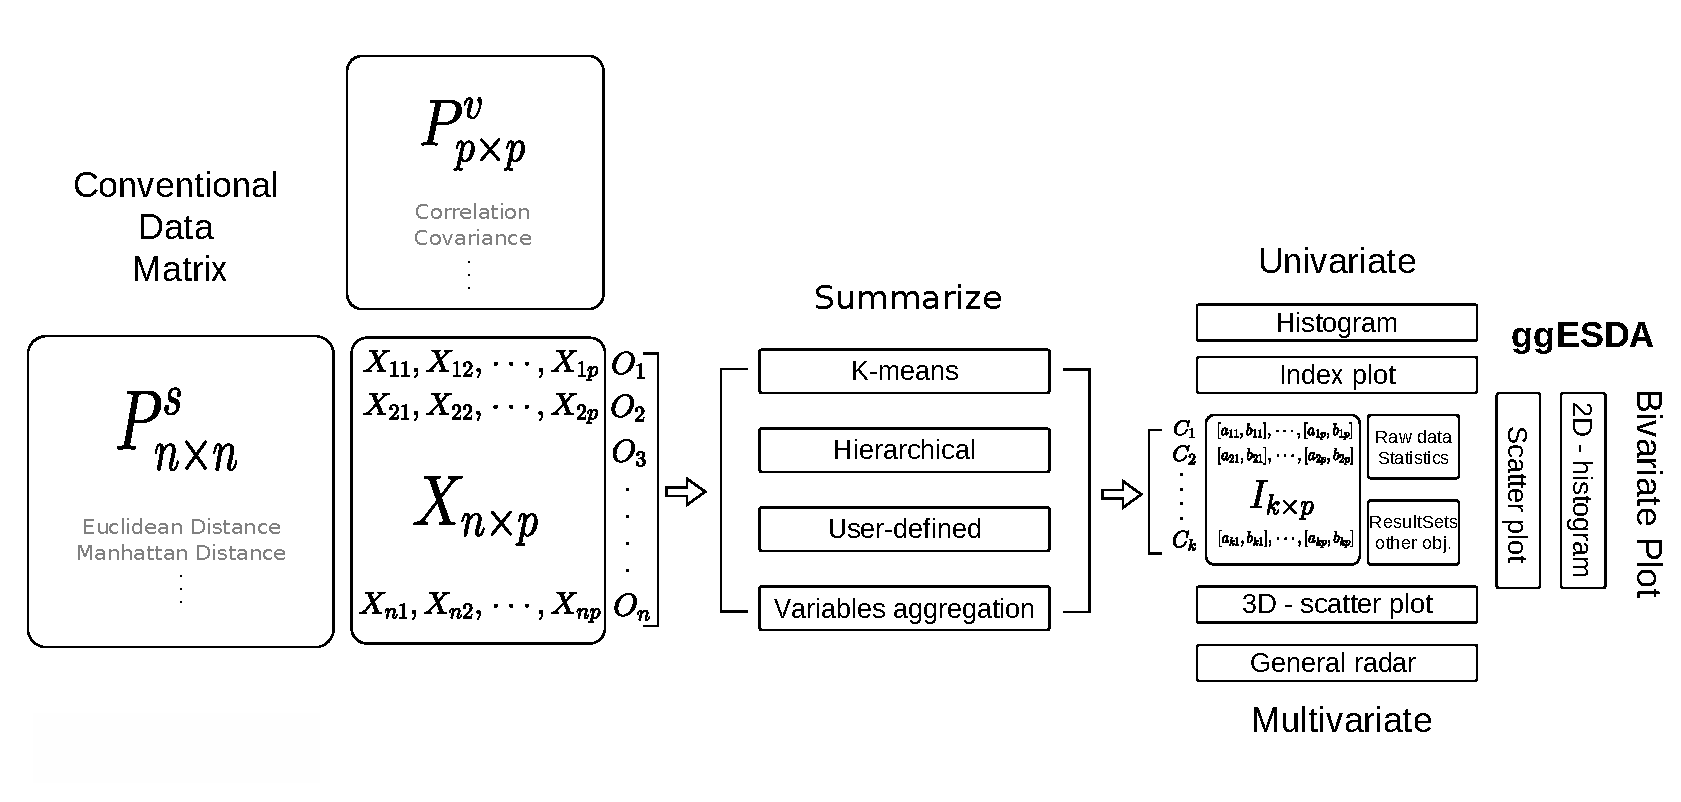
\includegraphics[width=1\textwidth]{doc/packageStructure2.eps} 
  		\caption{Package Structure and Diagram for the Transformation Flow} 
  		\label{fig:pkgStr}   			 		 
\end{figure}

As illustrated in Figure \ref{fig:pkgStr}, each row (observation) in the conventional data matrix $X_{p \times p}$ contains a vector of numeric values, $O_i = (x_1,x_2,\cdots,x_n)$, while each row of the interval-valued data matrix $I_{k \times p}$ contains a vector of intervals(ranges), $C_j = ([a_{j1},b_{j1}],[a_{j2},b_{j2}],\cdots,[a_{jp},b_{jp}])$, called a CONCEPT (or UNIT). The CONCEPT describe the behavior of a group of observations. Thus, the aggregation method between them is an essential process in SDA.

\subsection{Features}

\subsection{Datasets and Functionality}




\section{Application to Real Symbolic Datasets}

The typical graphical techniques of EDA include the index plot, barplot, boxplot, and histogram for univariate data; the 2D scatterplot, joint histogram and double boxplot for bivariate data; and the satterplot matrix, and star plot for multivariate data. Of course, there are many other variants of graphical techniques have been proposed. Our aim in this study is to implement good statistical graphics to display symbolic data accurately and clearly. 

\subsection{Example datasets}

In the following, to illustrate some graphing functions we have implemented so far, we will use the two well-known symbolic datasets. One is face recognition data (\cite{leroy:1996}; \cite{douzal:2011}; \cite{le:2012}). The dataset gives six face measurements of nine men (Figure \ref{fig:face}), each with three observations, resulting in a total 27 observations. The measurements for each observation came from a sequence of over 1,000 images. They cover a range of values, hence interval-valued variables. 

\begin{figure}[htbp]
\centering
\scalebox{.8}{
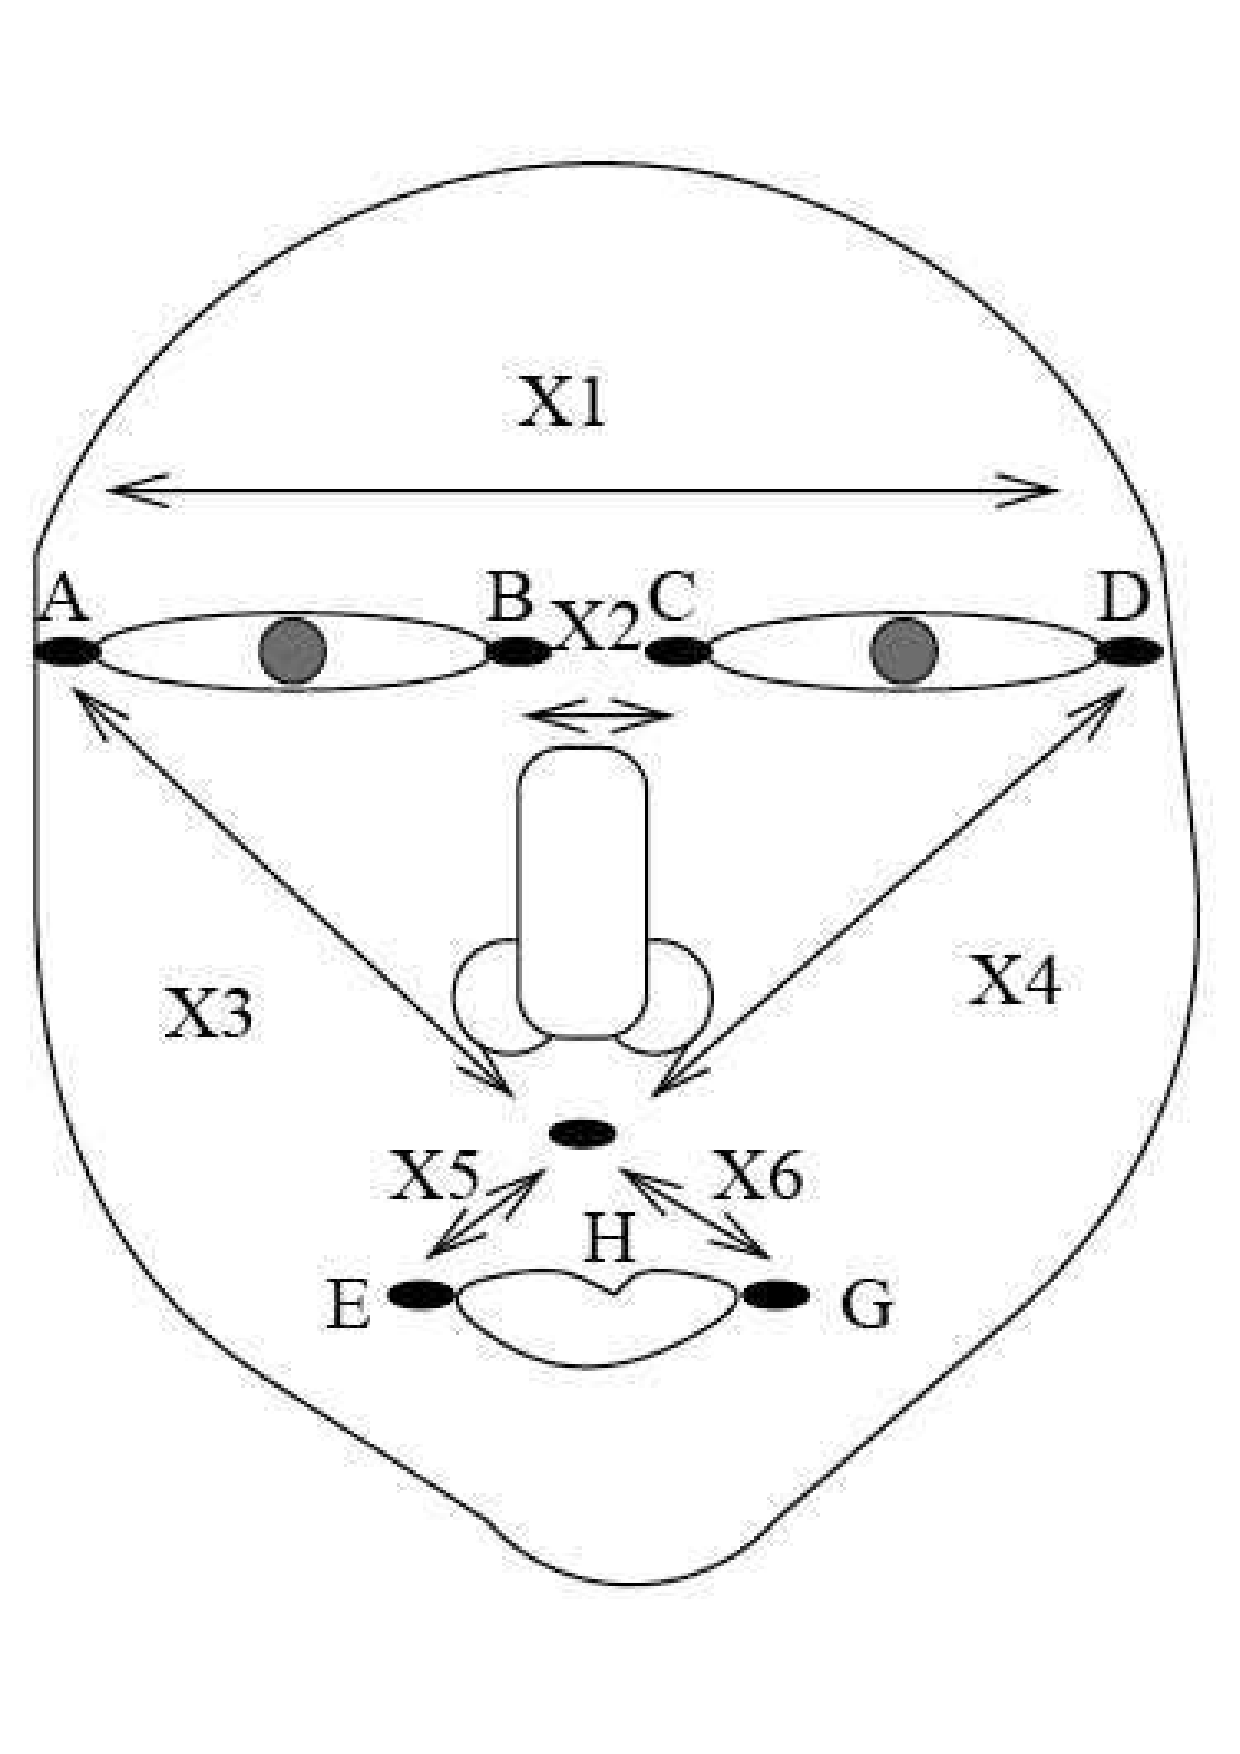
\includegraphics[width=0.4\textwidth]{face.pdf}
}
\caption{\label{fig:face} The six face measurements for the face recognition dataset}
\end{figure}

The other is the Environment questionnaire data (from the SODAS software package \cite{diday:2008}). Because of the demonstration of the performance dealing with modal multi-valued data, the same datasets were used in the radar plot. This dataset contains 14 objects and 17 variables and 4 of them are modal multi-valued, while the rest are interval-valued variables. Both of the part of example datasets are shown as follow:

\begin{Schunk}
\begin{Sinput}
> facedata[1:4, 1:4]
\end{Sinput}
\begin{Soutput}
# A tibble: 4 x 4
                 AD              BC                AH                DH
         <symblc_n>      <symblc_n>        <symblc_n>        <symblc_n>
1 [155.00 : 157.00] [58.00 : 61.01] [100.45 : 103.28] [105.00 : 107.30]
2 [154.00 : 160.01] [57.00 : 64.00] [101.98 : 105.55] [104.35 : 107.30]
3 [154.01 : 161.00] [57.00 : 63.00]  [99.36 : 105.65] [101.04 : 109.04]
4 [168.86 : 172.84] [58.55 : 63.39] [102.83 : 106.53] [122.38 : 124.52]
\end{Soutput}
\begin{Sinput}
> Environment[1:4, 4:6]
\end{Sinput}
\begin{Soutput}
# A tibble: 4 x 3
              REGIONDEVELOPME             CONTROL            SATISFY
                   <symblc_m>          <symblc_n>         <symblc_n>
1 4:0.47 3:0.25 2:0.19 1:0.09 [-723.25 : -339.65] [-133.91 : 250.83]
2 4:0.49 3:0.32 2:0.08 1:0.10  [-243.86 : 203.99] [-134.15 : 314.80]
3 4:0.56 3:0.22 2:0.18 1:0.04   [-195.44 : 90.10]  [-75.00 : 191.17]
4 4:0.64 3:0.21 2:0.14 1:0.01  [-279.12 : 120.61]  [342.58 : 705.03]
\end{Soutput}
\end{Schunk}

%\subsection{Univariate functions}

\subsection{Interval presentation techniques}

For interval-valued data, one of the advanced graphics implemented is called the min-max plot, which shows the interval characteristics of the data. As Figure \ref{fig:minmax} shown, we visualize the Face data for example by the function 

\begin{verbatim}
ggInterval_minmax(data = NULL, mapping = aes(NULL), scaleXY = "local",
  plotAll = FALSE)
\end{verbatim}

For the top six of Figure \ref{fig:minmax} shows the difference between each location of concept in each variable through the 45-degree line, which is a relative position of the variable itself (by setting option \code{scaleXY = "local"}). And represents the range by the connected line between minimum and maximum. To design the widely-view exploratory graphic function like this instance, we apply the option \code{plotAll = TRUE} to extend one variable visualization to full variables in the same plot. For examples, the figure constructed by the code

\begin{Schunk}
\begin{Sinput}
> relativePos <- ggInterval_minmax(facedata, plotAll = T, scaleXY = "local") +
+                scale_color_manual(values = c("darkblue", "darkred")) +
+                guides(colour = F) + 
+                theme_bw() + 
+                coord_fixed(ratio = 1)
> absolutePos <- ggInterval_minmax(facedata, plotAll = T, scaleXY = "local") +
+                scale_color_manual(values = c("darkblue", "darkred")) +
+                guides(colour = F) + 
+                theme_bw() + 
+                coord_fixed(ratio = 1)
> ggarrange(relativePos, absolutePos, nrow = 2, ncol = 1)
\end{Sinput}
\end{Schunk}

\begin{figure}[htbp]
    \centering
    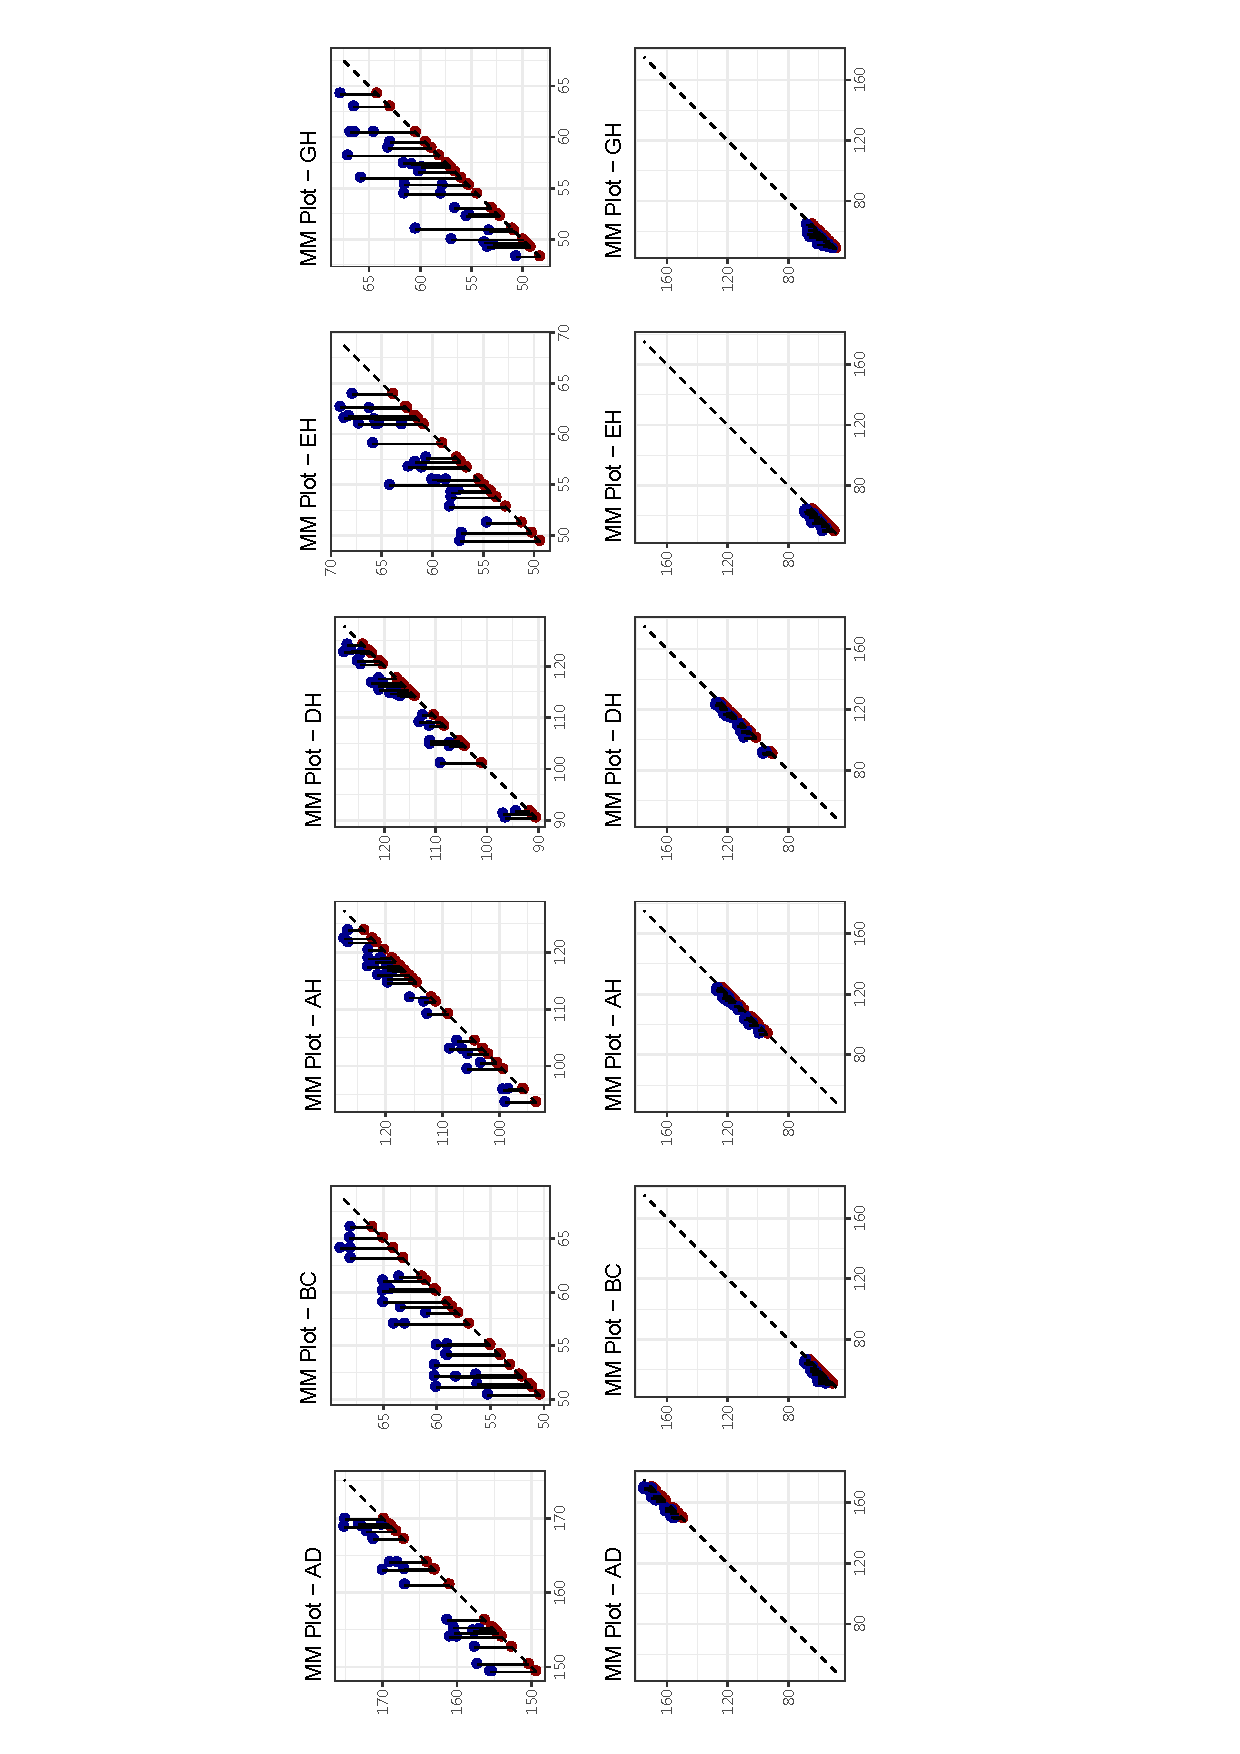
\includegraphics[trim=5cm 0.5cm 6cm 0.5cm,angle=-90,width=1\textwidth, clip]{mmplot.pdf} 
   \caption{\label{fig:minmax} The min-max plot. The figure in the top six conditions the axis in their own variables, whereas the bottom six conditions it in all variables.}
\end{figure}

However, when the unit is considered, the absolute position in the full sample space will display as the bottom six of Figure \ref{fig:minmax}. It presents a different boundary in the axis from the previous figure, which makes researchers know about the actual location in each variable. In this case, we can clearly discover that the sample space changes along with the variables.

To complete the visualization, it actually needs the command \code{ggInterval_minmax(facedata, plotAll = T, scaleXY = "local")}, merely. Other aesthetics can be omitted. Because we now focus on the full variables exploration, the \code{mapping} option for a particular variable is not necessary as well. Thus, in the following, we will pay more attention to the option we changing.



Another graphical technique, called index plot, is famous in conventional data as well. It is composed of minimum and maximum in interval-valued data and exhibits the concepts' behavior. Both of the function

\begin{verbatim}
ggInterval_index(data = NULL, mapping = aes(NULL))
\end{verbatim}

and 

\begin{verbatim}
ggInterval_indexImage(data = NULL, mapping = aes(NULL), plotAll = FALSE,
  column_condition = TRUE, full_strip = FALSE)
\end{verbatim}

can achieve this objective, but there is still a slight difference for visualizing. 

Take the variable AD for example, and set option \code{mapping = aes(x = AD)}. The former function, shown in Figures \ref{fig:index} and \ref{fig:index_bar}, directly displays the interval which is similar to min-max plot. Among these plots, we classify the concepts by the same person by setting the aesthetics option \code{fill} and can discover the values of people LOT, KHA, INC, FRA in AD variable are less than others, which easily compares the difference. 

The latter function, shown in Figure \ref{fig:image} and \ref{fig:image_full}, visualizes the interval values using a color mapping. As the legend says, the blue color corresponds to the low values, whereas the red color corresponds to the high. The only difference among these plots is the color bar extension (control by the option \code{full_strip = TRUE}), which will quickly discover concepts' behavior through the visual sense, as Figure \ref{fig:indexImage} shown.

\begin{figure}[htbp]
    \centering
    \scalebox{0.7}{
    \begin{tabular}{c c}
        \subfloat[Index plot]{
        \scalebox{.5}{
        \label{fig:index}
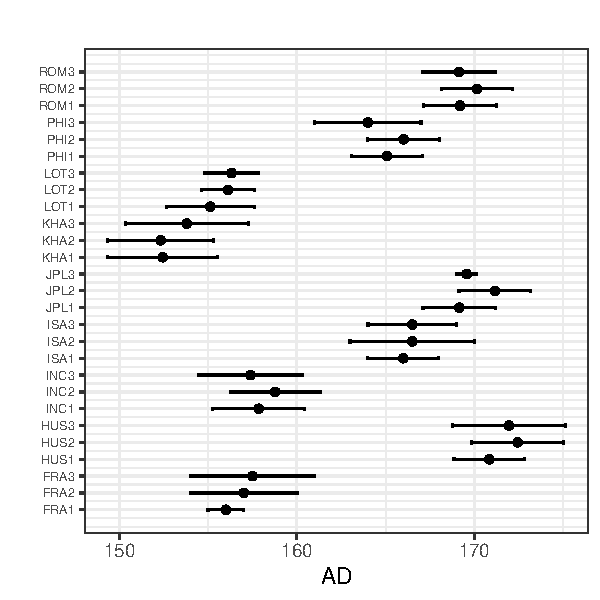
\includegraphics{ggESDA_Jiang&Wu_20210915-index}
                }}
                &
      
        \subfloat[Index plot with different group and common mean]{
        \scalebox{.5}{
        \label{fig:index_bar}
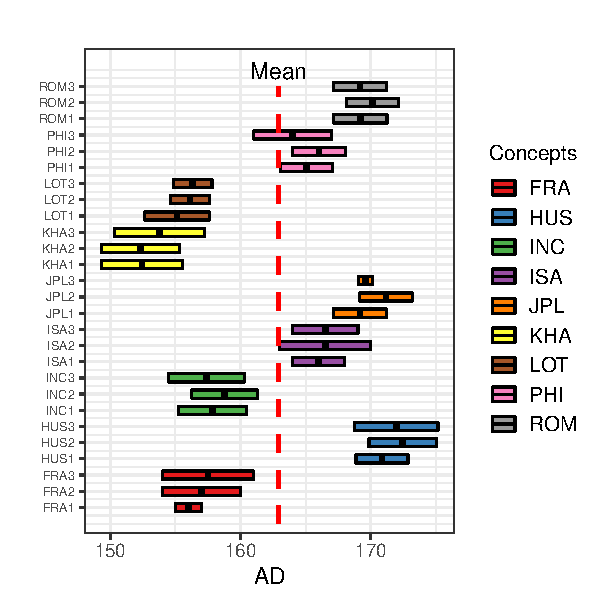
\includegraphics{ggESDA_Jiang&Wu_20210915-index_bar}
        }}
        \\
        
                \subfloat[Index image]{
                \scalebox{.5}{
                \label{fig:image}
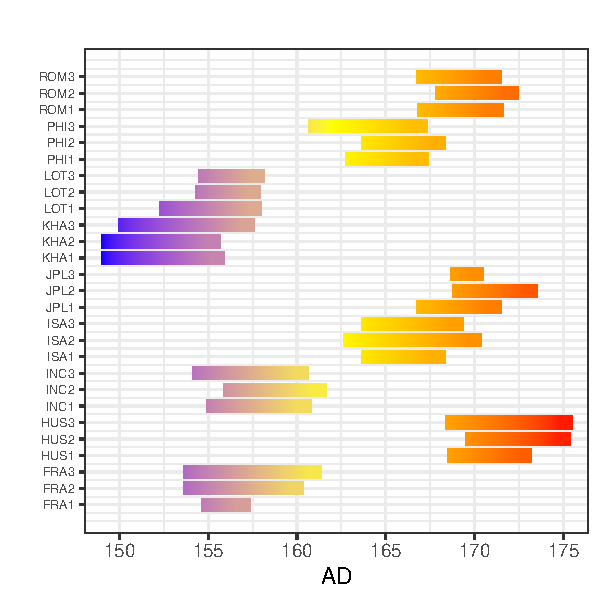
\includegraphics{ggESDA_Jiang&Wu_20210915-index_image1}
                }}
                &
        
        \subfloat[Index image with extended color]{
        \scalebox{.5}{
        \label{fig:image_full}
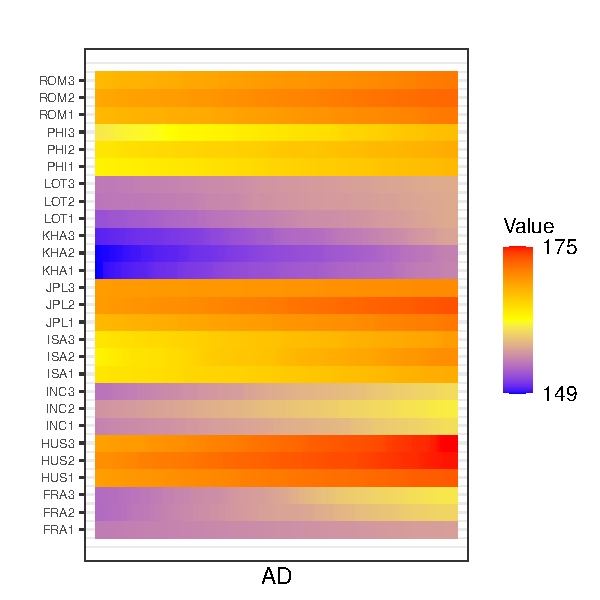
\includegraphics{ggESDA_Jiang&Wu_20210915-index_image2}
        }}
        \end{tabular}}
   \caption{\label{fig:index_full} Index plot for the variable AD}
\end{figure}

For exploring data, we extend the index plot into full variables and visualize by color mapping as we did before using the code

\begin{Schunk}
\begin{Sinput}
> colCondition <- ggInterval_indexImage(facedata, plotAll = T,
+                                       full_strip = T) 
> matCondition <- ggInterval_indexImage(facedata, plotAll = T,
+                                       full_strip = T,
+                                       column_condition = F)
> ggarrange(colCondition, matCondition, nrow = 1, ncol = 2)
\end{Sinput}
\end{Schunk}

\begin{figure}[htbp]
    \centering
    \scalebox{1}{
    \begin{tabular}{c c}
        \subfloat[Column condition]{
        \scalebox{.5}{
        \label{fig:indexImage_col}
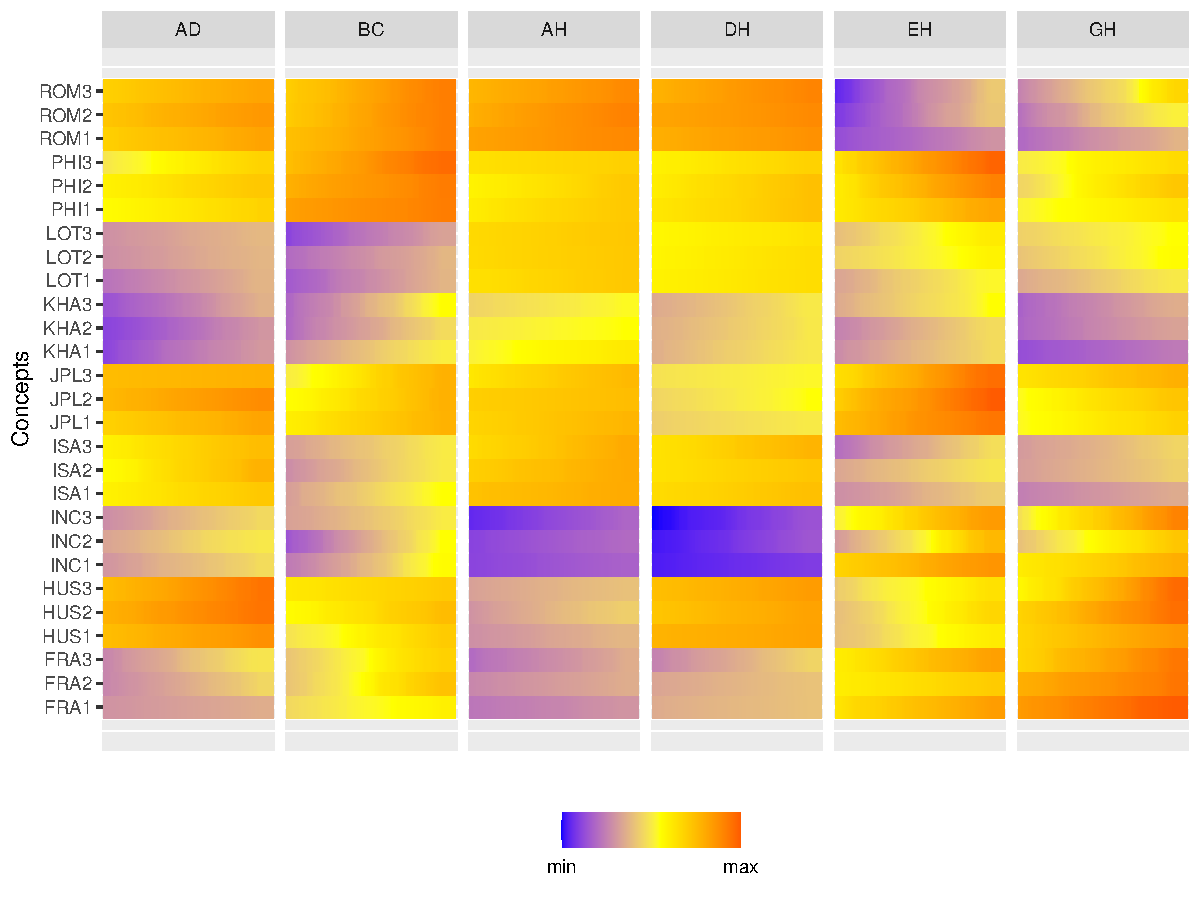
\includegraphics{ggESDA_Jiang&Wu_20210915-indexImage_col}
                }}
                &
        \subfloat[Matrix condition]{
        \scalebox{.5}{
        \label{fig:indexImage_mat}
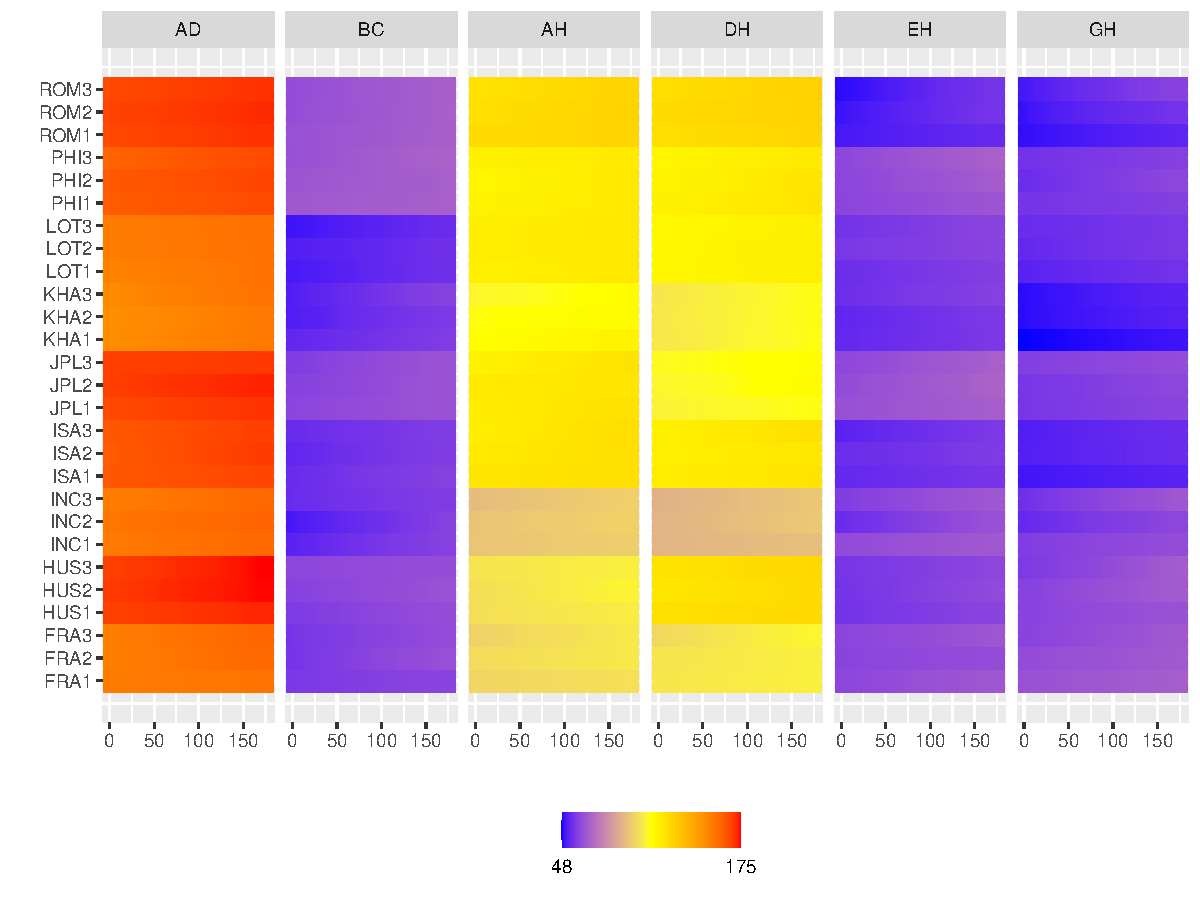
\includegraphics{ggESDA_Jiang&Wu_20210915-indexImage_mat}
        }}
        \end{tabular}}
    \caption{\label{fig:indexImage} Index image - heatmap}
\end{figure}

Figure \ref{fig:indexImage} shows two kinds of presentation ways for this method.

\begin{itemize}
  \item \emph{Column condition}: This technique is to standardize data by each variable, which will be able to compare the observations easily without the unit confounder. Figure \ref{fig:indexImage_col} ,for example, shows the concept JPL has a large value in all variables in contrast with KHA and INC.
  \item \emph{Matrix condition}: Instead of standardizing variables one by one, this method does it with the full data matrix. That will reveal the different performance between each variable, as Figure \ref{fig:indexImage_mat} shown. The values in variable AD are obviously larger than others, which means the interocular distance is the longest than other distances in the face dataset.
\end{itemize}


\subsection{Statistical graph implementation}

In this field, it reveals the trend, distribution, how large the data spread, etc, for a particular variable. Moreover, another advanced graphics implemented is called center-range plot, which helps researchers to be able to grasp the relationship between center and range. 

The side-by-side boxplot, which provides a quick view of data distribution, dispersion, and is particularly useful for comparing distributions between several groups of variables. Use the function

\begin{verbatim}
ggInterval_boxplot(data = NULL, mapping = aes(NULL), plotAll = FALSE)
\end{verbatim}

By setting option \code{plotAll}, the top panel of Figure \ref{fig:box} will be easily implemented. In this Figure, the dispersion of six variables is obviously distinct. However, it is difficult to compare with their distribution because of the distinct sample space which leaves no room for a suitable presentation. We standardize the Face data, shown in the bottom panel of the figure, and take a deeper look at it.

\begin{figure}[htbp]
    \centering
    \scalebox{0.8}{
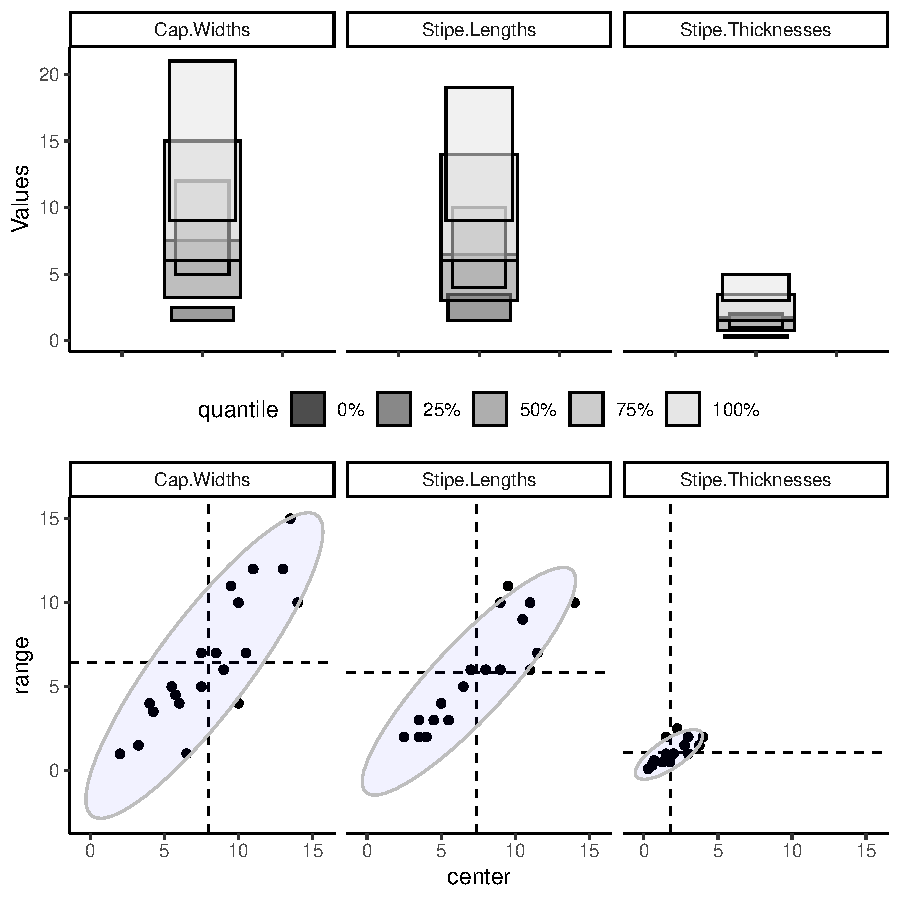
\includegraphics{ggESDA_Jiang&Wu_20210915-box_centerRange_before}
    }
    \caption{The side-by-side box plot. The figure in the top panel is the raw value of its variables, where the bottom panel is to standardize each variables. \label{fig:box}}
\end{figure}

Clearly, there is a vacancy in the middle of variable AD, AH, and next to the minimum of the variable DH, which indicates the frequency there may be quite low. Especially for AD and AH, this factor may result in a bimodal distribution.

In addition, the overlap of the variables BC, EH, and GH located in the middle of five quantile-box seem larger than others, which is possible to lead a bell-shaped for its distribution.

% center range
For the center-range plot, it is a special technique for the dispersion observing. The code

\begin{verbatim}
ggInterval_centerRange(data = NULL, mapping = aes(NULL), plotAll = FALSE)
\end{verbatim}

Setting options are the same as the former. With the Figure \ref{fig:box} demonstration, we divide the exploration into two parts by standardization, shown in Figure \ref{fig:centerRange}.

With regard to the top panel of Figure \ref{fig:centerRange}, there is no significant difference in the range of all variables. But focusing on a particular variable, the dispersion is quite large. For the bottom panel of Figure \ref{fig:centerRange}, the relationship between center and range is clearly exposed. Among them, there is an obvious relationship in the variable BC, which presents a negative correlation, where others are not significant.

\begin{figure}[htbp]
    
    \centering
    \scalebox{0.8}{
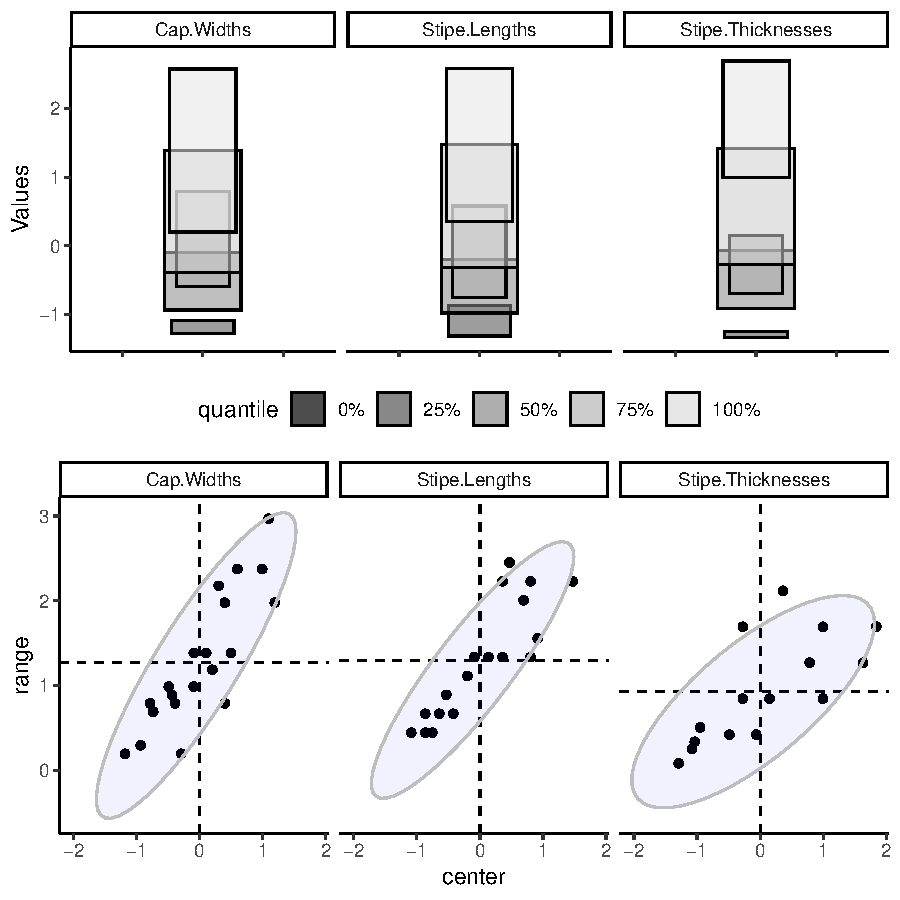
\includegraphics{ggESDA_Jiang&Wu_20210915-box_centerRange_after}
    }
    \caption{\label{fig:centerRange}The center-range plot}
\end{figure}


In the same way, demonstrating the distribution of data by histogram is also one of the most common ways. Construct the frequency of data by Section \ref{sec:hist} for the first, which will be processed by the function

\begin{verbatim}
ggInterval_hist(data = NULL, mapping = aes(NULL), method = "equal-bin",
  bins = 10, plotAll = FALSE)
\end{verbatim}

Option \code{method} is the key for setting whether the histogram bins are equal width, detail in Section \ref{sec:hist}, which can be set with \code{"equal-bin"} or \code{"unequal-bin"}. In Figure \ref{fig:hist} depicts the histograms with equidistant and non-equidistant breaks for all six variables. Both of them present the location and scale of distribution of each variable, but the non-equidistant-bin histogram whose breaks are obtained by the boundaries of the intervals shows more details about the characteristic of data. As we did before, set \code{plotAll} and \code{method}, and it can be directly completed with one line command. In the figure, we may obtain some similar distribution information conclusion with Figure \ref{fig:box}.

\begin{figure}[htbp]
    \centering
    \scalebox{0.9}{
    \begin{tabular}{c c}
        \subfloat[Equidistant-bin histogram]{
        \scalebox{.5}{
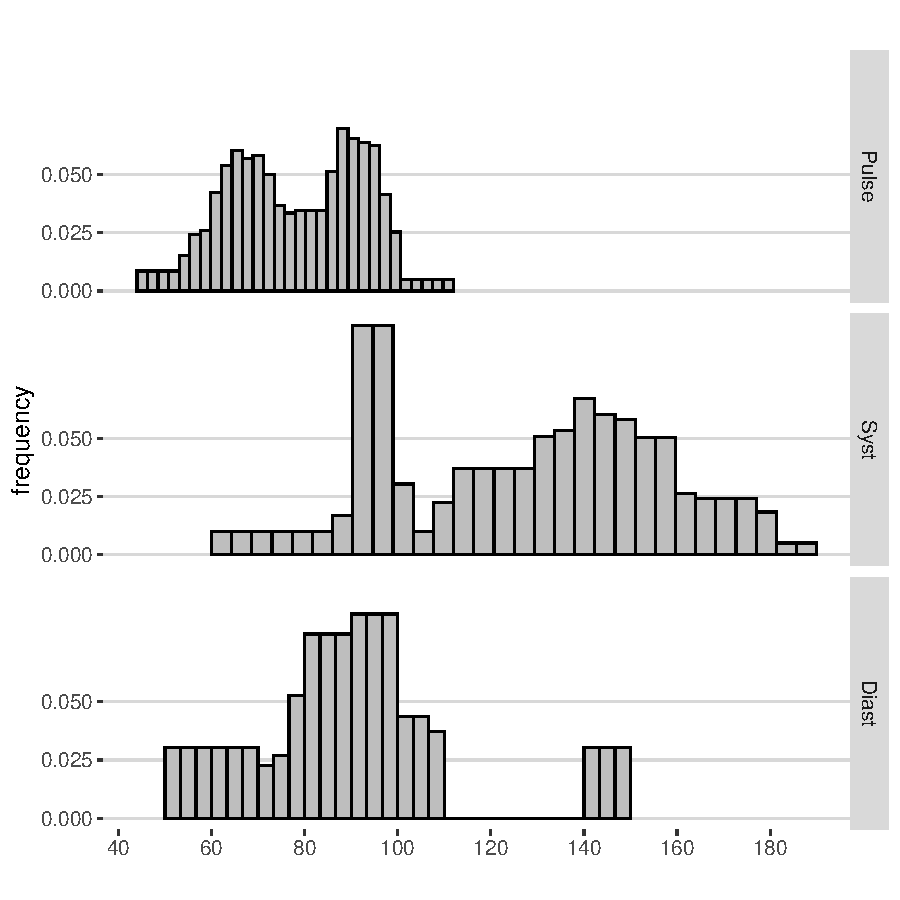
\includegraphics{ggESDA_Jiang&Wu_20210915-hist_equal}
                }}
                &
        \subfloat[Non-equidistant-bin histogram]{
        \scalebox{0.5}{
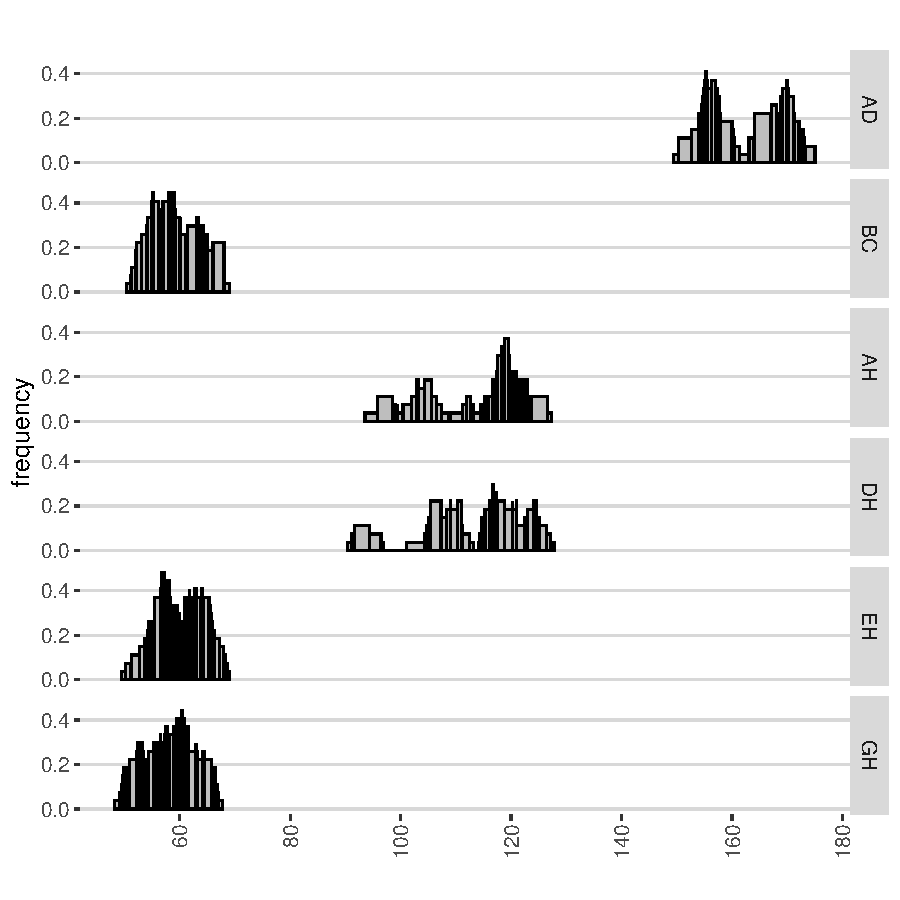
\includegraphics{ggESDA_Jiang&Wu_20210915-hist_unequal}
        }}
        \end{tabular}}
    \caption{\label{fig:hist} Histogram}
\end{figure}





%\subsection{Bivariate functions}

\subsection{Bivariate relationship plot}

The bivariate functions reveal relationships between variables, trends of the regression line, and joint frequency across the sample space. In this field, we design the scatter plot, two-dimension histogram, and also implement the most well-known approach, the vertices method of principal component analysis (V-PCA) \cite{cazes1997extension}. Additionally, these graphic techniques can visualize multiple variables at the same time by matrix type.

For instance, the code of scatter matrix of Figure \ref{fig:scaMatrix}:

\begin{Schunk}
\begin{Sinput}
> ggInterval_scaMatrix(data = facedata)+
+   theme_bw()+
+   theme(legend.position = "none")
\end{Sinput}
\end{Schunk}

\begin{figure}[htbp]
\centering
\scalebox{0.9}{
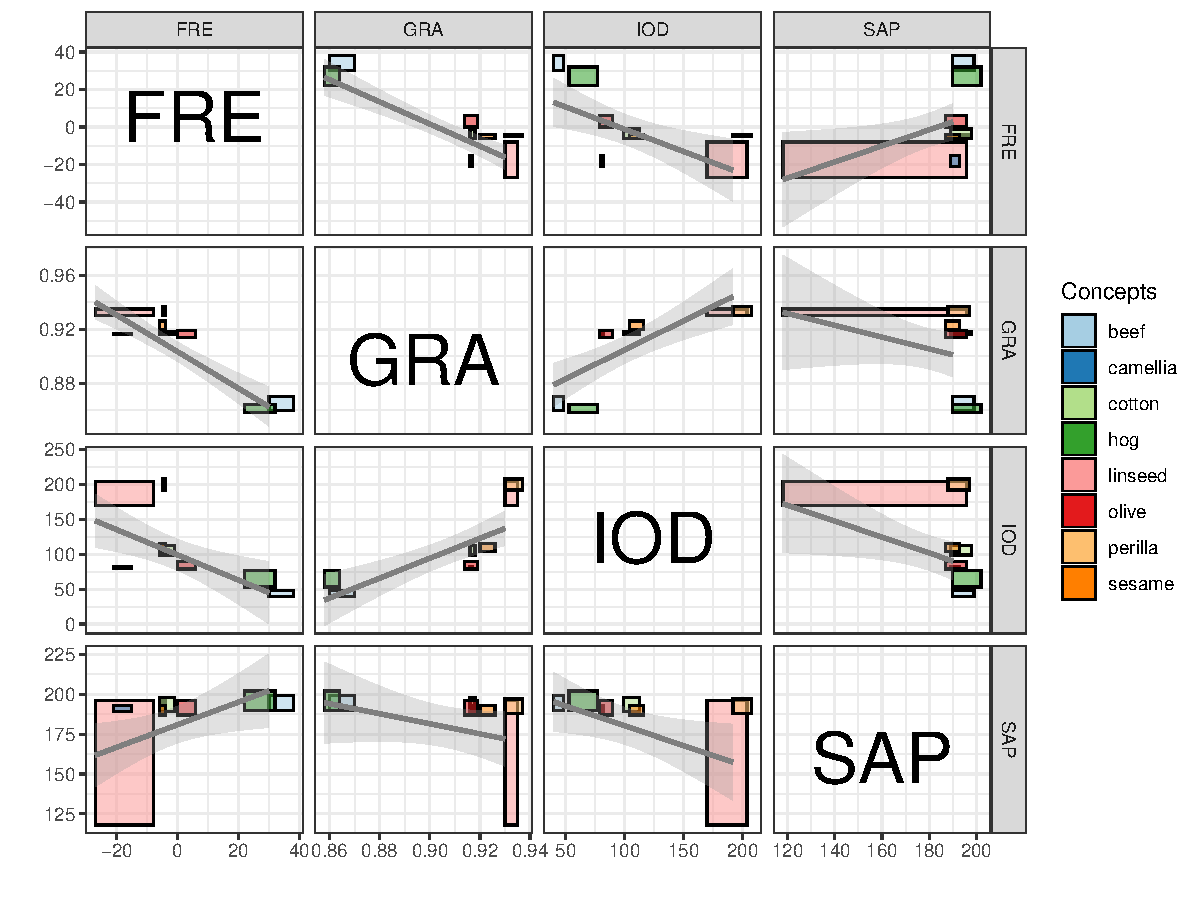
\includegraphics{ggESDA_Jiang&Wu_20210915-scaMatrix}
}
\caption{\label{fig:scaMatrix} scatter matrix}
\end{figure}


In Figure \ref{fig:scaMatrix}, we use grayscale to represent the concepts and the rectangle to display the intersection of two interval-valued observations. The relationship among this graph is clearly depicted. The variables AH and DH are an obvious positive correlation, whereas AD and AH seems to be an exponential relation. Of course, there is an easy way for scatter plot of two particular variables using the function \code{ggInterval_scatter}. With the technique, we can implement the maximum covering area rectangle (MCAR) \cite{cazes1997extension}, which is widely used for graphical representation of interval objects on a DR (dimension reduction) subspace, owing to its simplicity, shown as Figure \ref{fig:mcar}. Nevertheless, the main drawback of MCAR is that the interval objects are oversized in the DR subspace with respect to the real objects in $\mathbb{R}^p$, hence, the polytopes representation \cite{le2012symbolic} for interval data was proposed. 

Although PCA methods are widely applied in \proglang{R}, we still develop the graphic function for them using 

\begin{verbatim}
ggInterval_PCA(data = NULL, mapping = aes(NULL), plot = TRUE, poly = FALSE, 
  concepts_group = NULL)
\end{verbatim}

The control option of PCA visualization method mentioned above is \code{poly}, which can be set with \code{TRUE} for the polytopes representation as shown in Figure \ref{fig:poly}. By the dimension reduction and color mapping on each person, Figure \ref{fig:PCA} shows most of the concepts are clearly separated.

\begin{figure}[htbp]
    \centering
    \scalebox{0.8}{
    \begin{tabular}{c c}
        \subfloat[Vertice-PCA (MCAR)]{
        \scalebox{.6}{
        \label{fig:mcar}
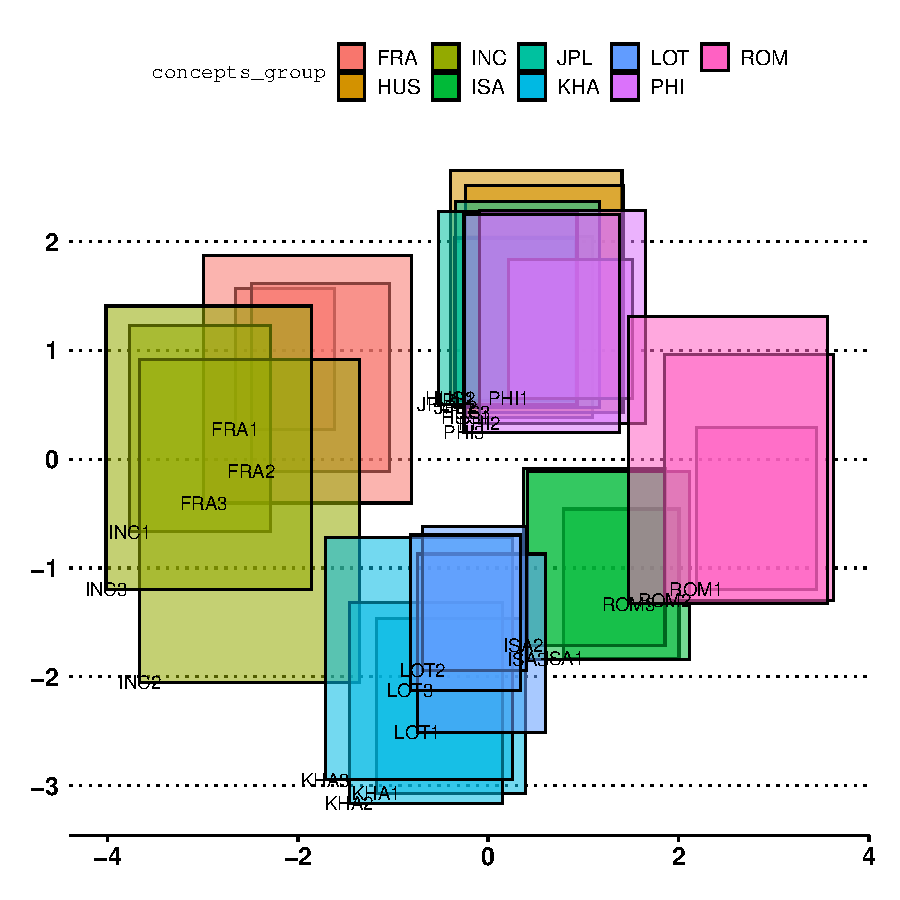
\includegraphics{ggESDA_Jiang&Wu_20210915-PCA_MCAR}
                }}
                &
        \subfloat[Vertice-PCA (Polytope)]{
        \scalebox{.6}{
        \label{fig:poly}
        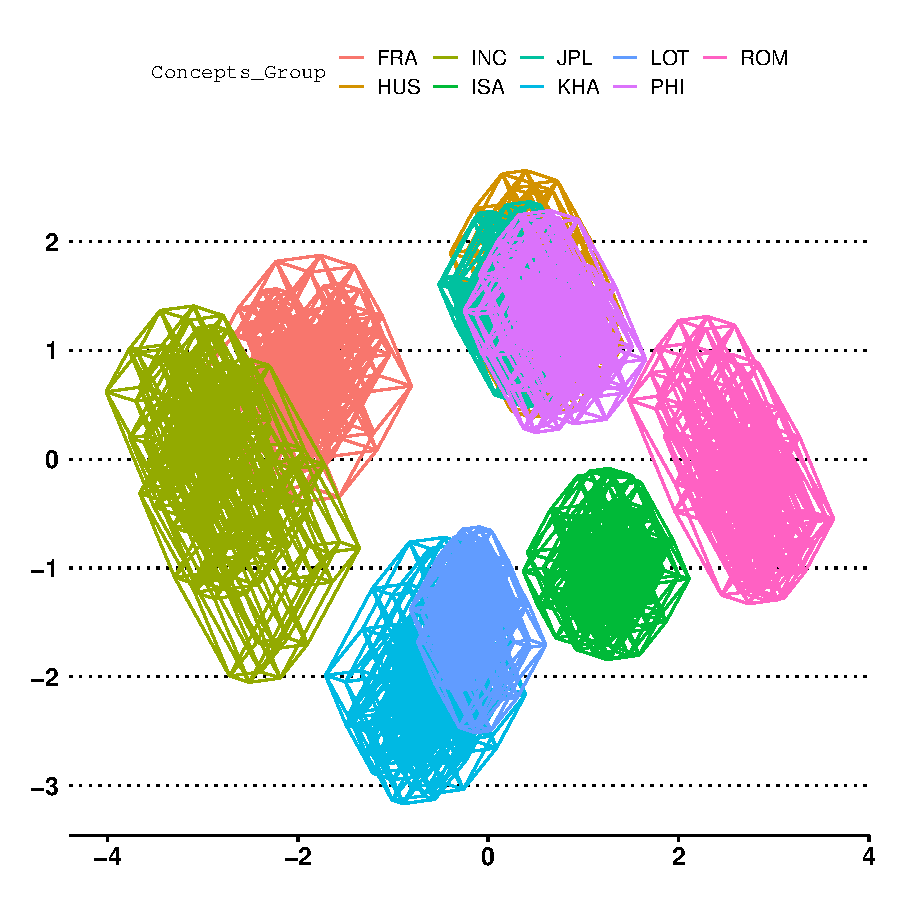
\includegraphics[]{ggESDA_Jiang&Wu_20210915-PCA_Polytope.pdf
}
        }}
        \end{tabular}}
    \caption{\label{fig:PCA} Two kinks of PCA for interval-valued data, where the XY-axis are represent the first principal component and the second principal component, respectively.}
\end{figure}

Another bivariate relationship plot is two-dimension histogram, which is to calculate joint histogram frequency (details in Section \ref{sec:hist2d}) and using matrix visualization (\cite{chen2002generalized}; \cite{chen2004matrix}) to plot. The code

\begin{Schunk}
\begin{Sinput}
> ggInterval_2Dhist(facedata, aes(x = AD, y = BC, col = "grey30"),
+                   xBins = 25, yBins = 25) + 
+   theme_light() +
+   theme(legend.position = "bottom") + 
+   coord_fixed(ratio = 1)
\end{Sinput}
\end{Schunk}


uses the joint frequency between the variables AD and BC and makes the XY-axis bins partial into 25 subintervals. As Figure \ref{fig:2Dhist} shown, we can observe that the concepts in these joint sample spaces concentrate on the top-right and bottom-left areas that seem like a slightly positive correlation.

\begin{figure}[htbp]
\centering
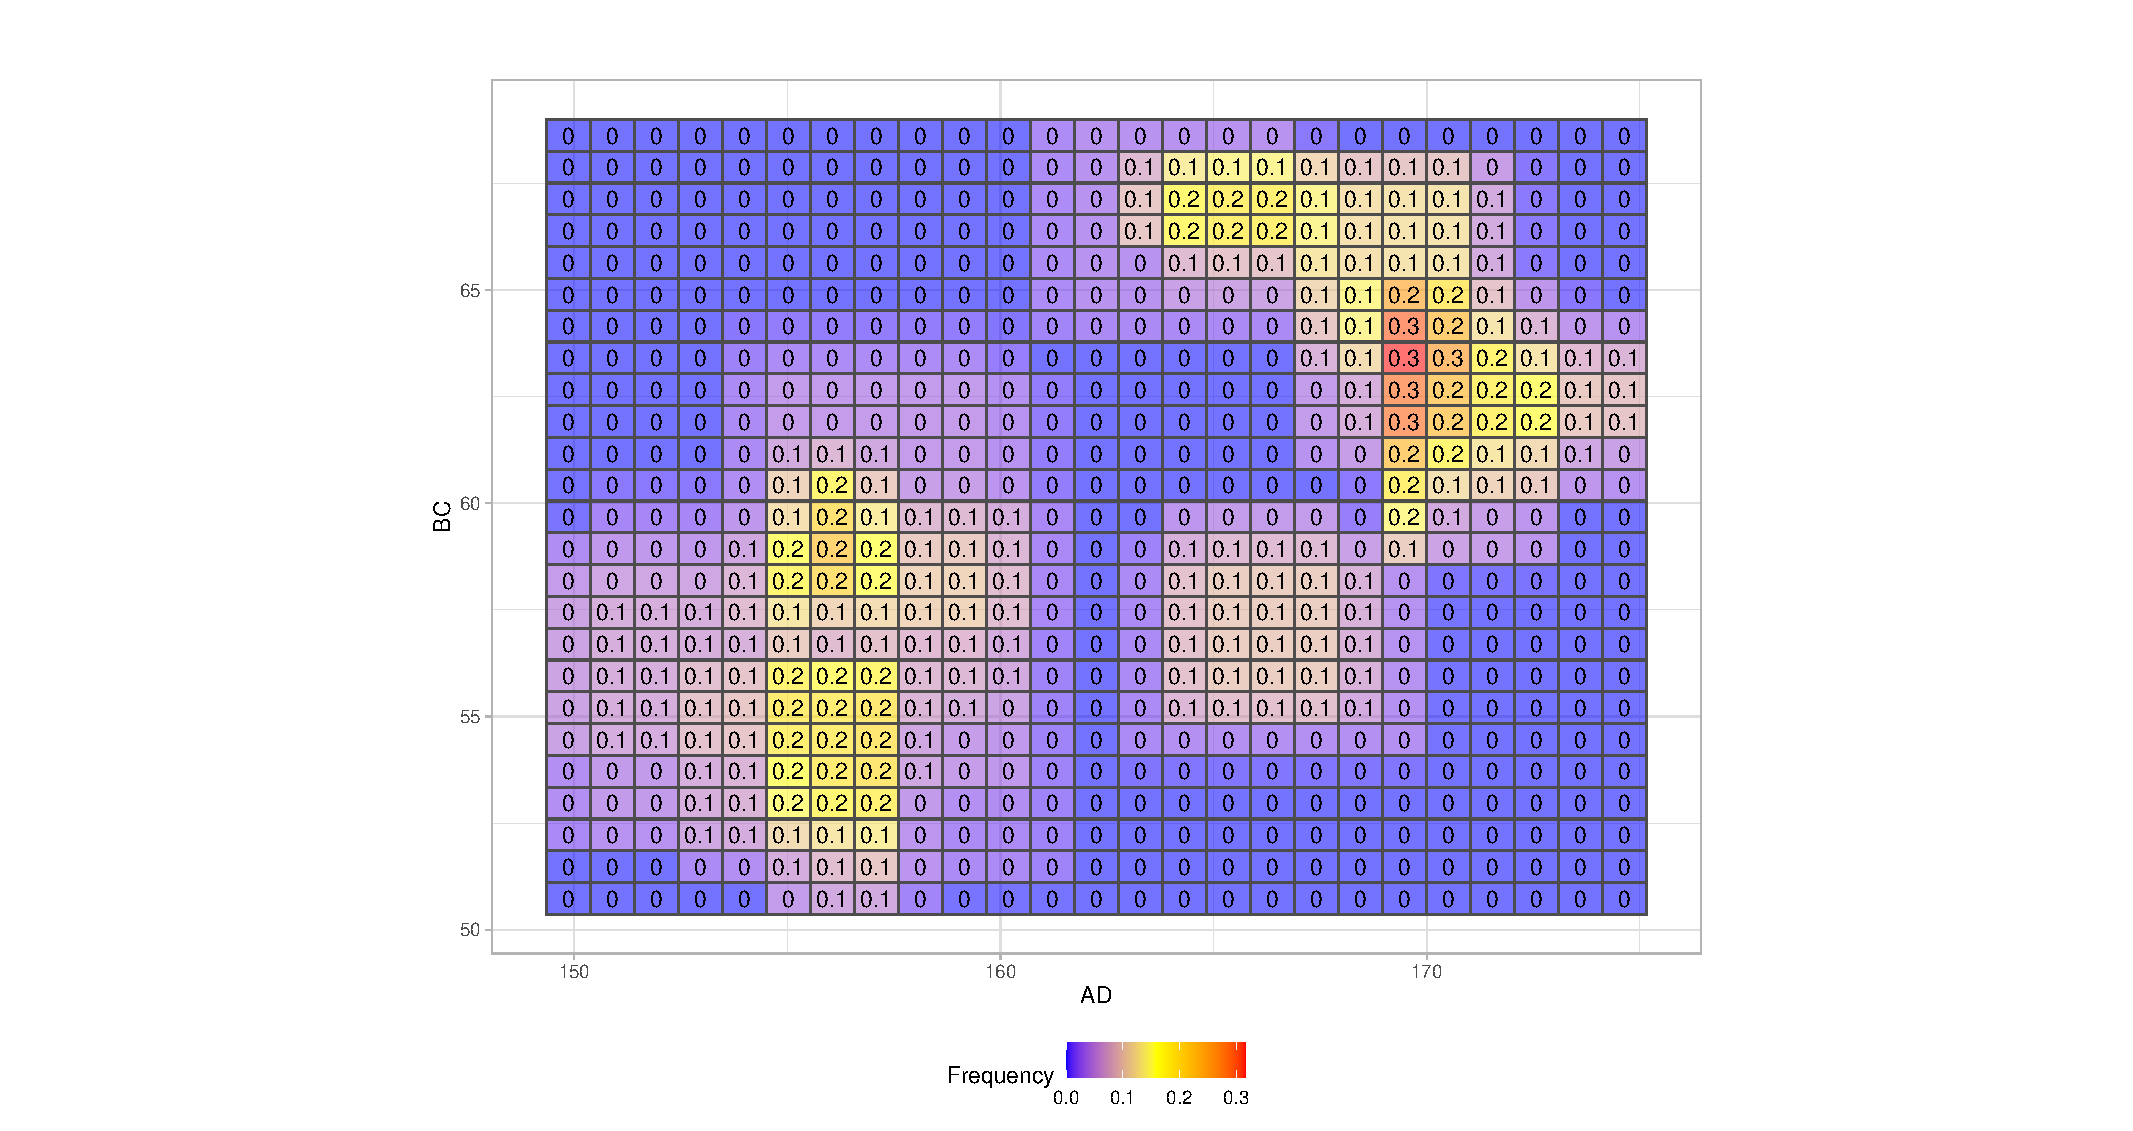
\includegraphics[width=0.8\textwidth]{ggESDA_Jiang&Wu_20210915-2Dhist.pdf
}
\caption{\label{fig:2Dhist} 2D histogram }
\end{figure}

In the same way, extend the plot to full variables as matrix type by the code

\begin{Schunk}
\begin{Sinput}
> ggInterval_2DhistMatrix(facedata, aes(col = "grey50"), xBins = 10,
+                         yBins = 10, removeZero = T, addFreq = F) + 
+   theme_light() + 
+   labs(title="") +
+   theme(legend.position = "bottom")
\end{Sinput}
\end{Schunk}

The addition options \code{removeZero} and \code{addFreq} make zero value and frequency displaying remove, shown as Figure \ref{fig:2DhistMatrix}. Not only the relationship presentation, the graphic technique also depicts the details frequency. Among these, we might get a similar conclusion between variables relation, but for the calculation, this technique may consume a larger time-complexity than scatter plot.

\begin{figure}[htbp]
\centering
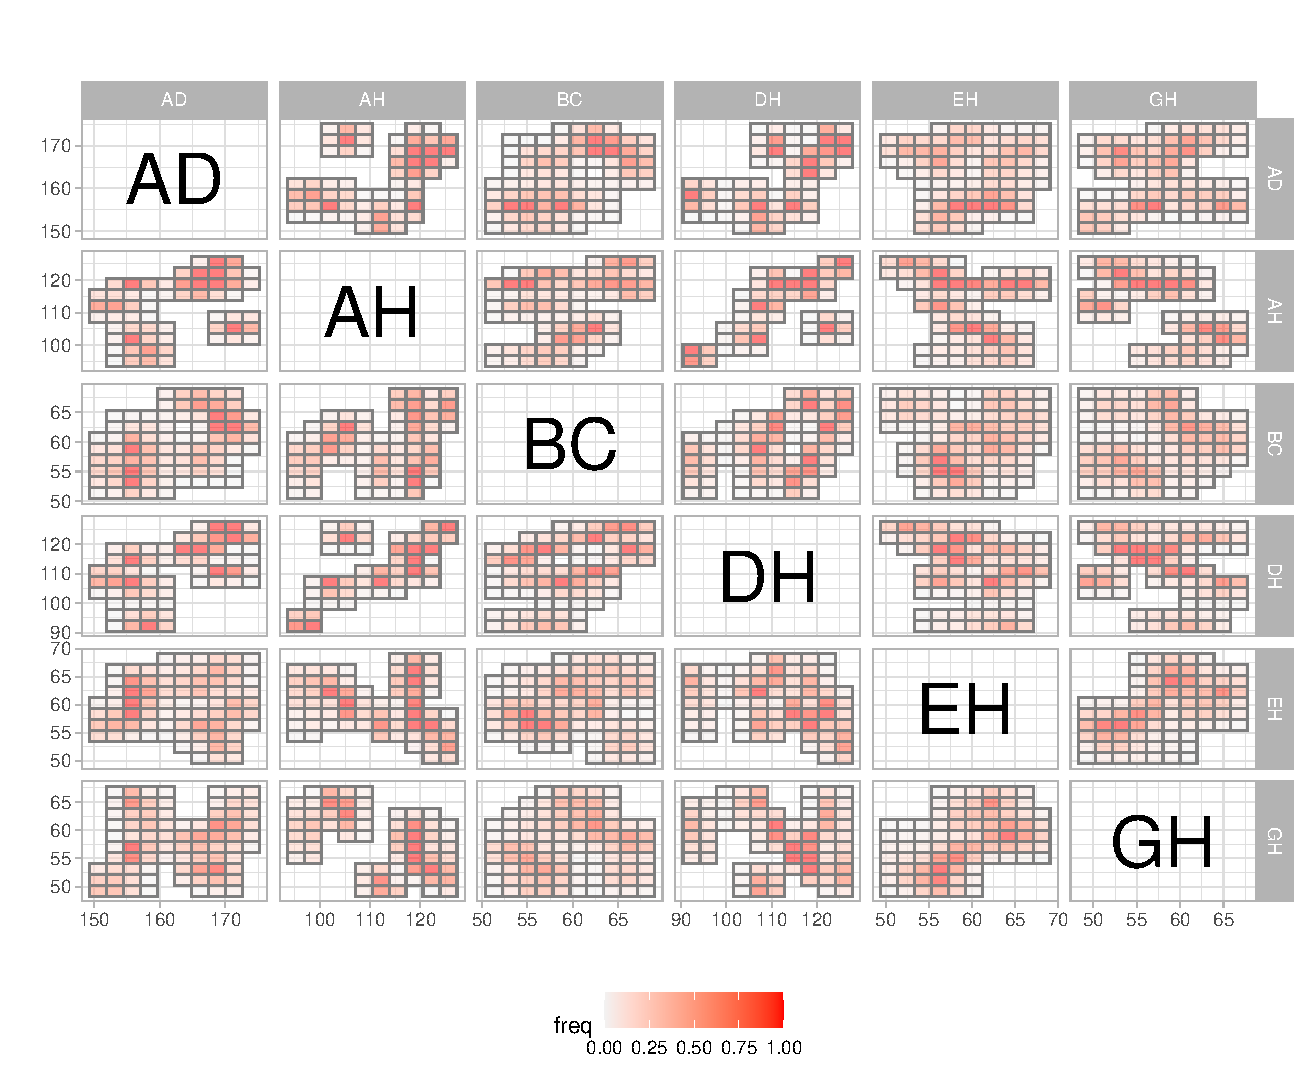
\includegraphics[width=0.9\textwidth]{ggESDA_Jiang&Wu_20210915-2DhistMatrix.pdf
}
\caption{\label{fig:2DhistMatrix} 2D histogram matrix}
\end{figure}


\subsection{Multivariate visualization}

In the field of multivariate visualization, the most common graphic technique is radar plot, also known as star plot. In \pkg{ggESDA}, we provide the function

\begin{verbatim}
ggInterval_radar(data = NULL, layerNumber = 3, inOneFig = TRUE, Drift = 0.5, 
  showLegend = TRUE, showXYLabs = FALSE, plotPartial = NULL, alpha = 0.5, 
  base_circle = TRUE, base_lty = 2, addText = TRUE, type = "default",
  quantileNum = 4, addText_modal = TRUE, addText_modal.p = FALSE)
\end{verbatim}

Except for the aesthetic options \code{layerNumber}, \code{showLegend}, \code{showXYLabs}, \code{alpha}, \code{base_circle}, \code{base_lty}, and \code{addText}, the visualizing key is to determine which concepts are presented through setting \code{plotPartial} with the rows of concepts. In addition, it will be decided to use area (\code{"default"}), rectangle (\code{"rect"}), or quantile (\code{"quantile"}) to represent the interval by option \code{type}.

Above all, take the Environmental questionnaire dataset for example, and the variety of typical multivariate radar plots for a specific concept is shown in Figure \ref{fig:radar_typical} by the code

\begin{Schunk}
\begin{Sinput}
> #Remove the modal multi-valued variables
> Environment.i <- Environment[, 5:17] #take interval-valued
> left.fig <- ggInterval_radar(Environment.i, plotPartial = 2,
+                              showLegend = F, addText = F) +
+             labs(title = "") +
+             theme_hc() 
> #Remain the modal multi-valued variables
> right.fig <- ggInterval_radar(Environment, plotPartial = 2,
+                               showLegend = F, base_circle = F,
+                               base_lty = 1) +
+              labs(title = "") +
+              theme_hc() +
+              scale_fill_manual(values = "gray50") +
+              scale_color_manual(values = "gray50") 
> gridExtra::marrangeGrob(list(left.fig, right.fig), 
+                         nrow = 1, ncol = 2, top = "")
\end{Sinput}
\end{Schunk}

\begin{figure}[htbp]
\centering
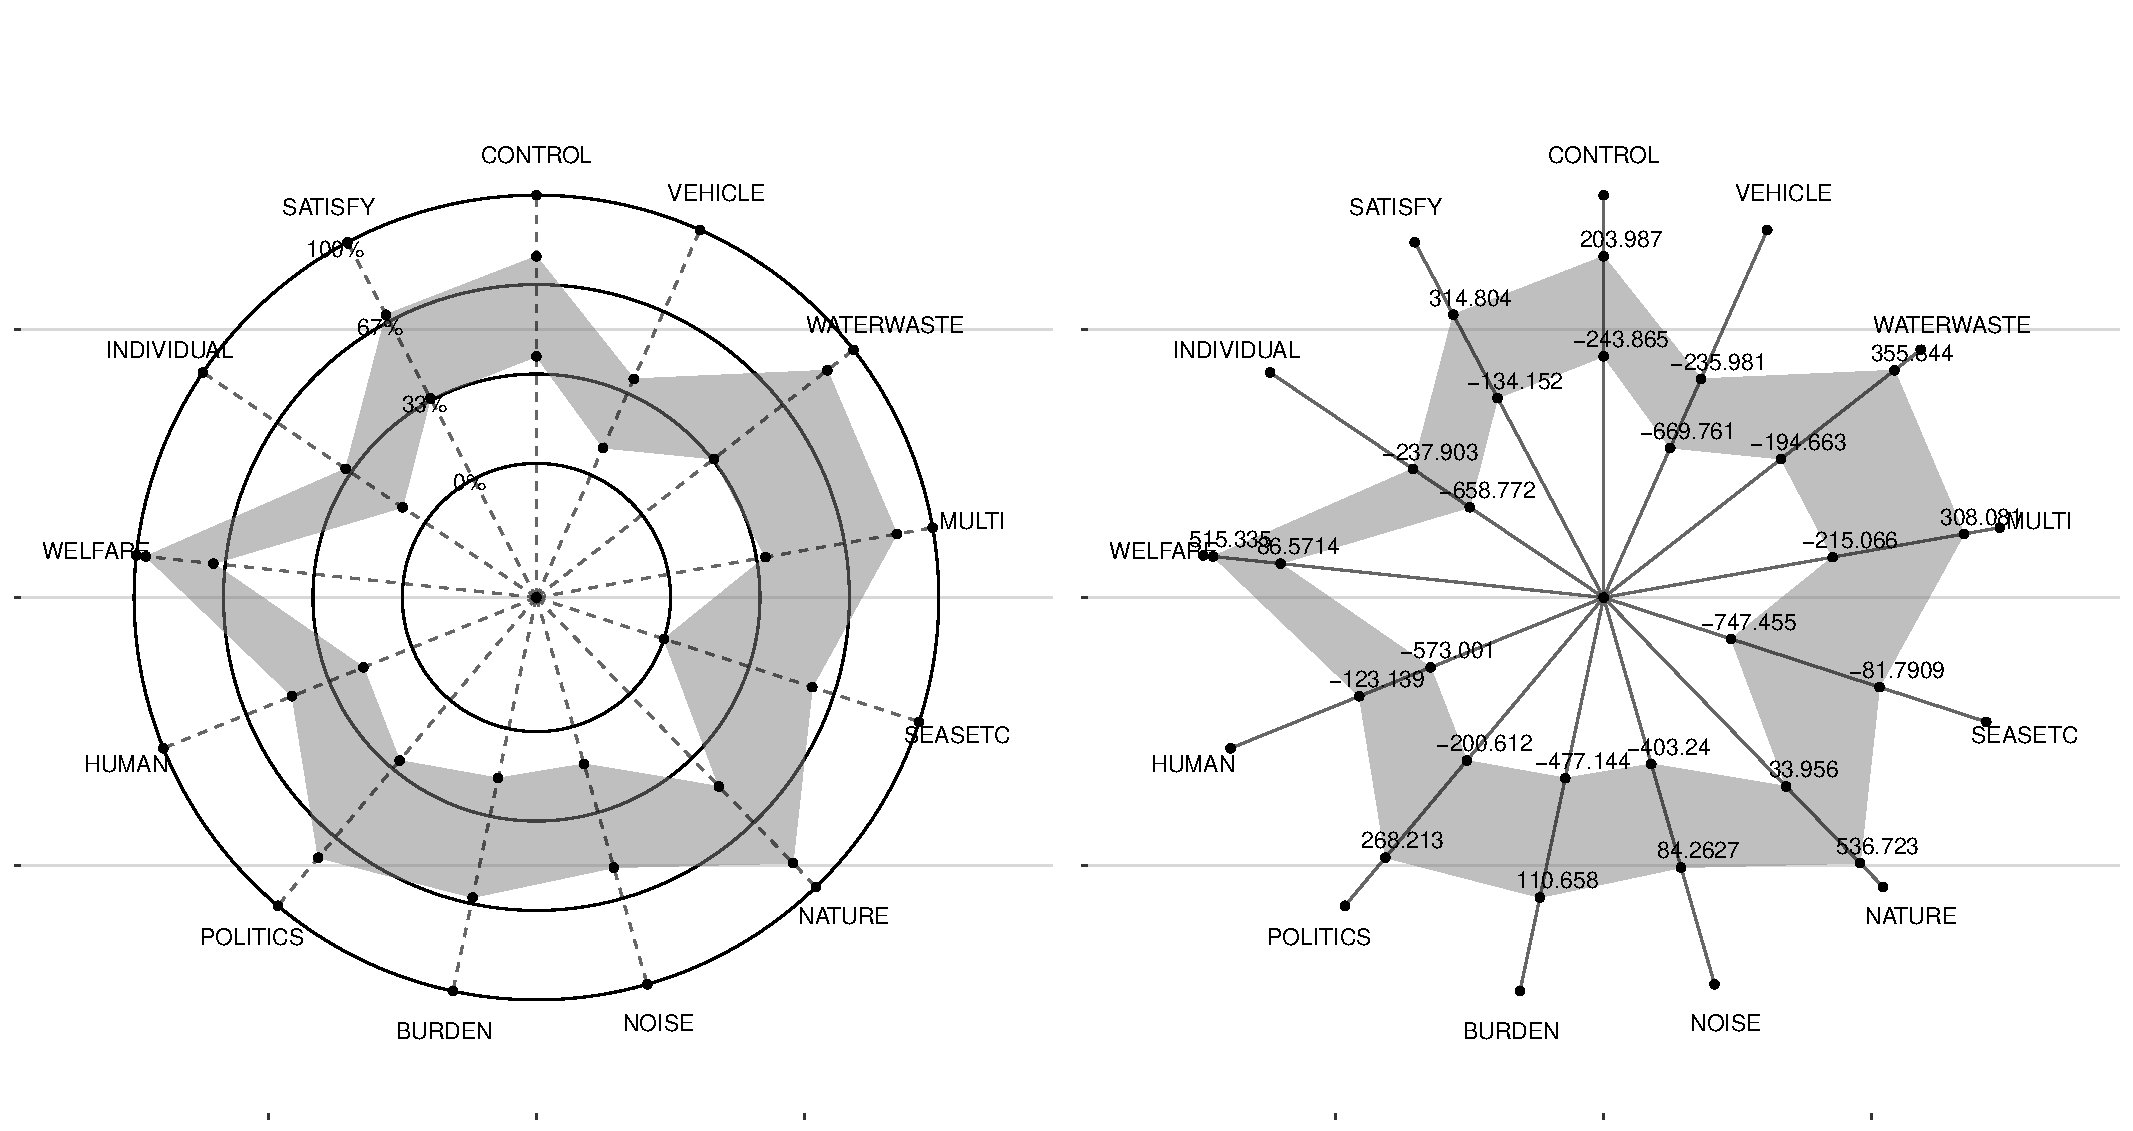
\includegraphics[width=0.9\textwidth]{radar_typical.pdf} 
\caption{\label{fig:radar_typical} The variety of typical radar plot which is able to contain interval-valued and modal multi-valued variables.}
\end{figure}

Use the color to represent the interval area, and it can clearly present the behavior of the particular concept in each variable. The figure in the left panel shows the relative position of the interval by the percentage circle, whereas the right one removes it and adds the frequency in the plot. Additionally, the kind of radar plot is generalized to visualize not only the interval-valued data but the modal multi-valued, which we design a cuboid to represent, and the height will correspond to the probability of the factor in the variable, as the right panel in the figure. The technique not just merges the distinct variable's type in one plot but even helps the researcher to compare with concepts easily under multiple variables. Figure \ref{fig:radar_3obs} shows the three observations presented by the different plot. 

\begin{figure}[htbp]
\centering
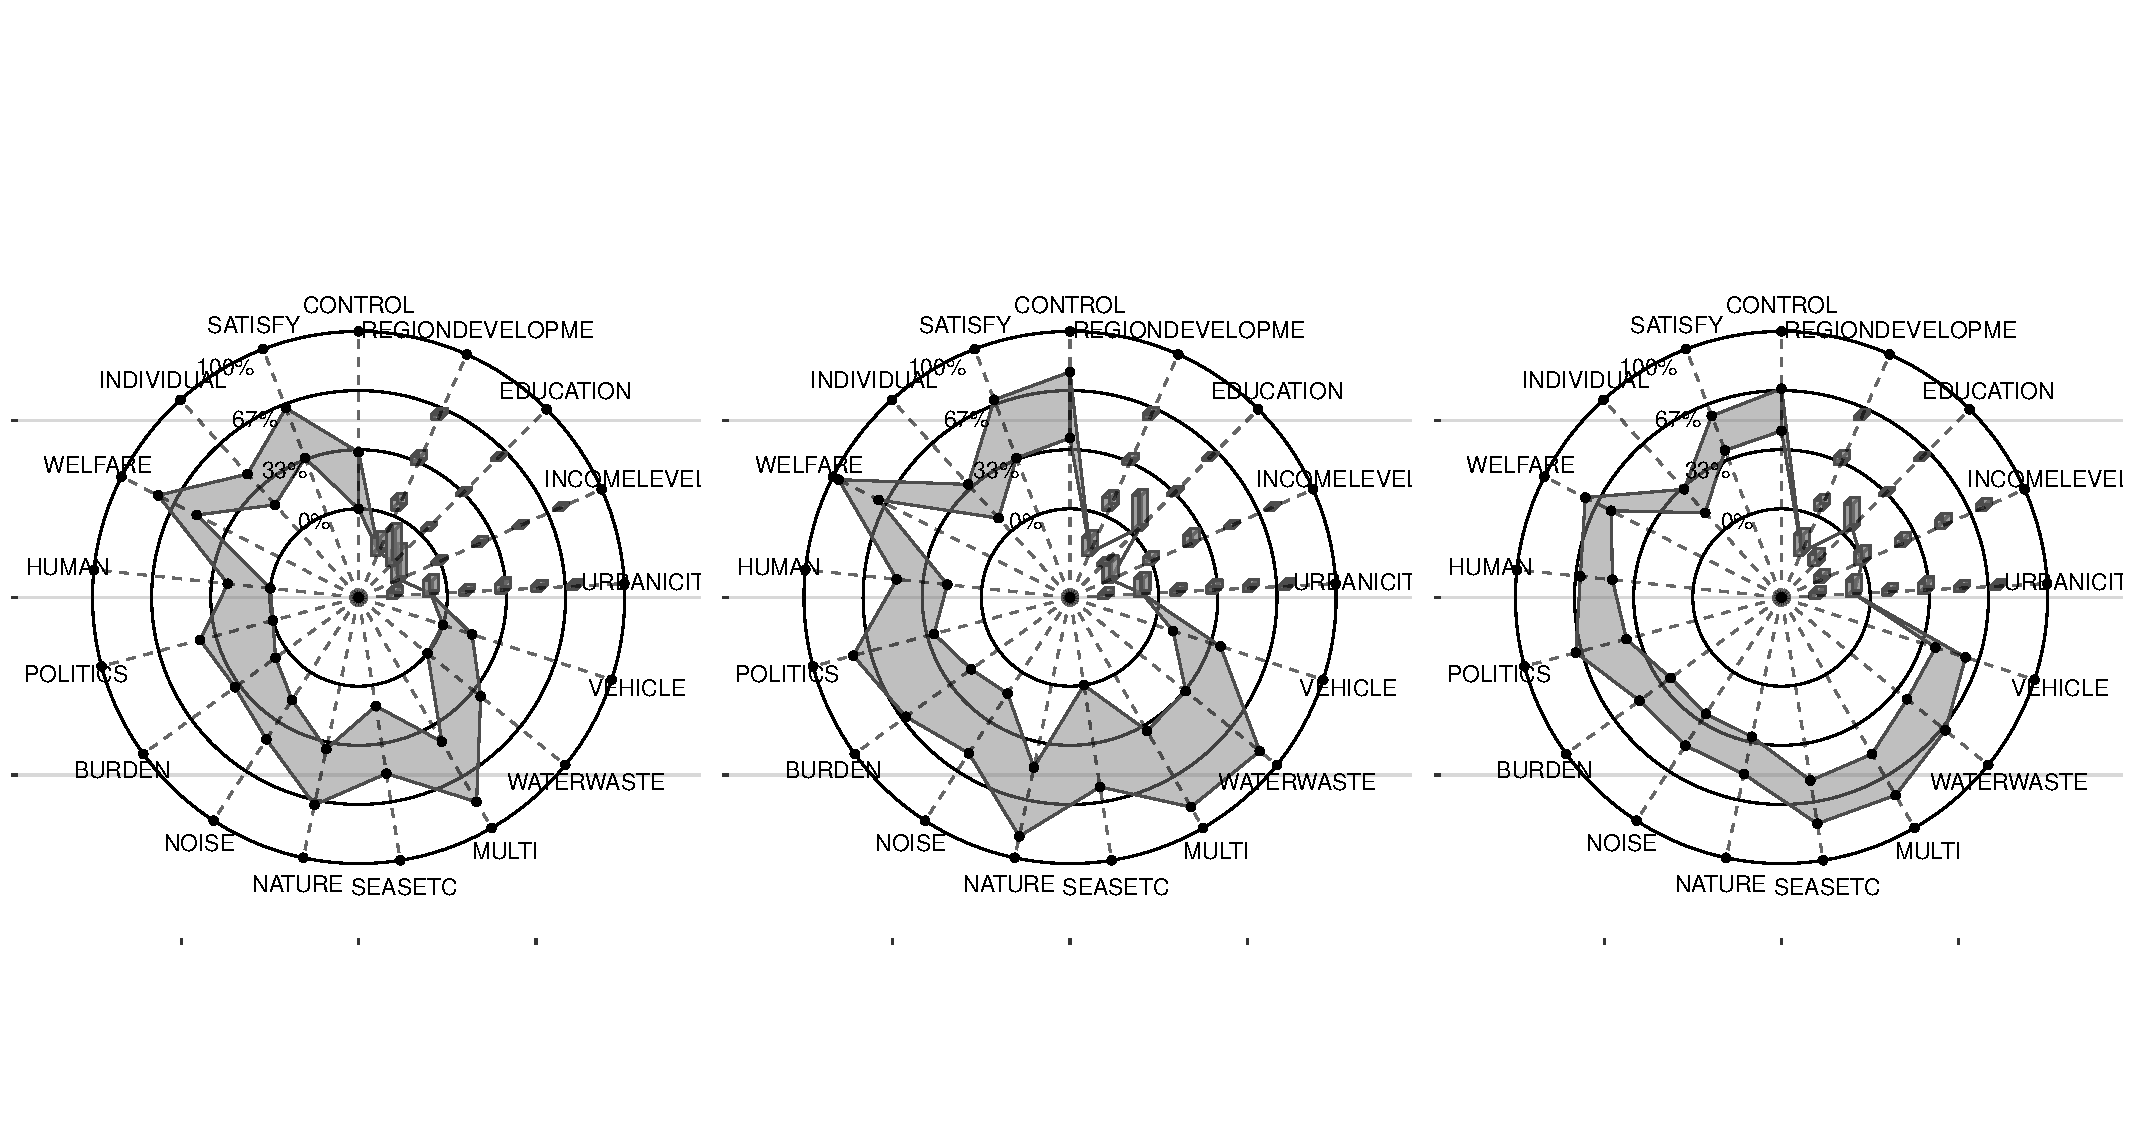
\includegraphics[trim=0cm 3cm 0cm 3cm,width=1\textwidth, clip]{radar_3obs.pdf} 
\caption{\label{fig:radar_3obs} Compare three distinct observations by multiple variables.}
\end{figure}

Moreover, another advanced implemented graphic technique of radar plot is classification by different concepts using a color mapping. By the code:
\begin{Schunk}
\begin{Sinput}
> area.fig <- ggInterval_radar(Environment, plotPartial = c(4, 6),
+                              showLegend = F, base_circle = F,
+                              base_lty = 1, addText = F,
+                              addText_modal = F) +
+             scale_fill_manual(values = c("darkred", "darkblue")) +
+             scale_color_manual(values = c("darkred", "darkblue")) +
+             labs(title = "") +
+             theme_hc()
> rect.fig <- ggInterval_radar(Environment, plotPartial = c(4, 6),
+                              showLegend = F, base_circle = F,
+                              base_lty = 1, addText = F, type = "rect",
+                              addText_modal = F) +
+             scale_fill_manual(values = c("darkred", "darkblue")) +
+             scale_color_manual(values = c("darkred", "darkblue")) +
+             labs(title = "") +
+             theme_hc()
> gridExtra::marrangeGrob(list(area.fig, rect.fig), 
+                         nrow = 1, ncol = 2, top = "")
\end{Sinput}
\end{Schunk}

we can get the Figure \ref{fig:radar}. It's worth mentioning that whenever the users determine the option \code{plotPartial} with multiple observations and set \code{inOneFig = TRUE} which means if pool observations into the same figure, the mechanism in the function will automatically classify by color. In this case, the two visualized concepts are represented by blue and red color, and the modal multi-valued variables are stacked by the same factor. On the contrast, the graph displays the interval-valued variables in two ways. The left panel of the figure shows a typical area-presenting way, while the right one use rectangle to show the interval. These implement can be completed by setting the option \code{type} with \code{"default"} and \code{"rect"} respectively.

\begin{figure}[htbp]
\centering
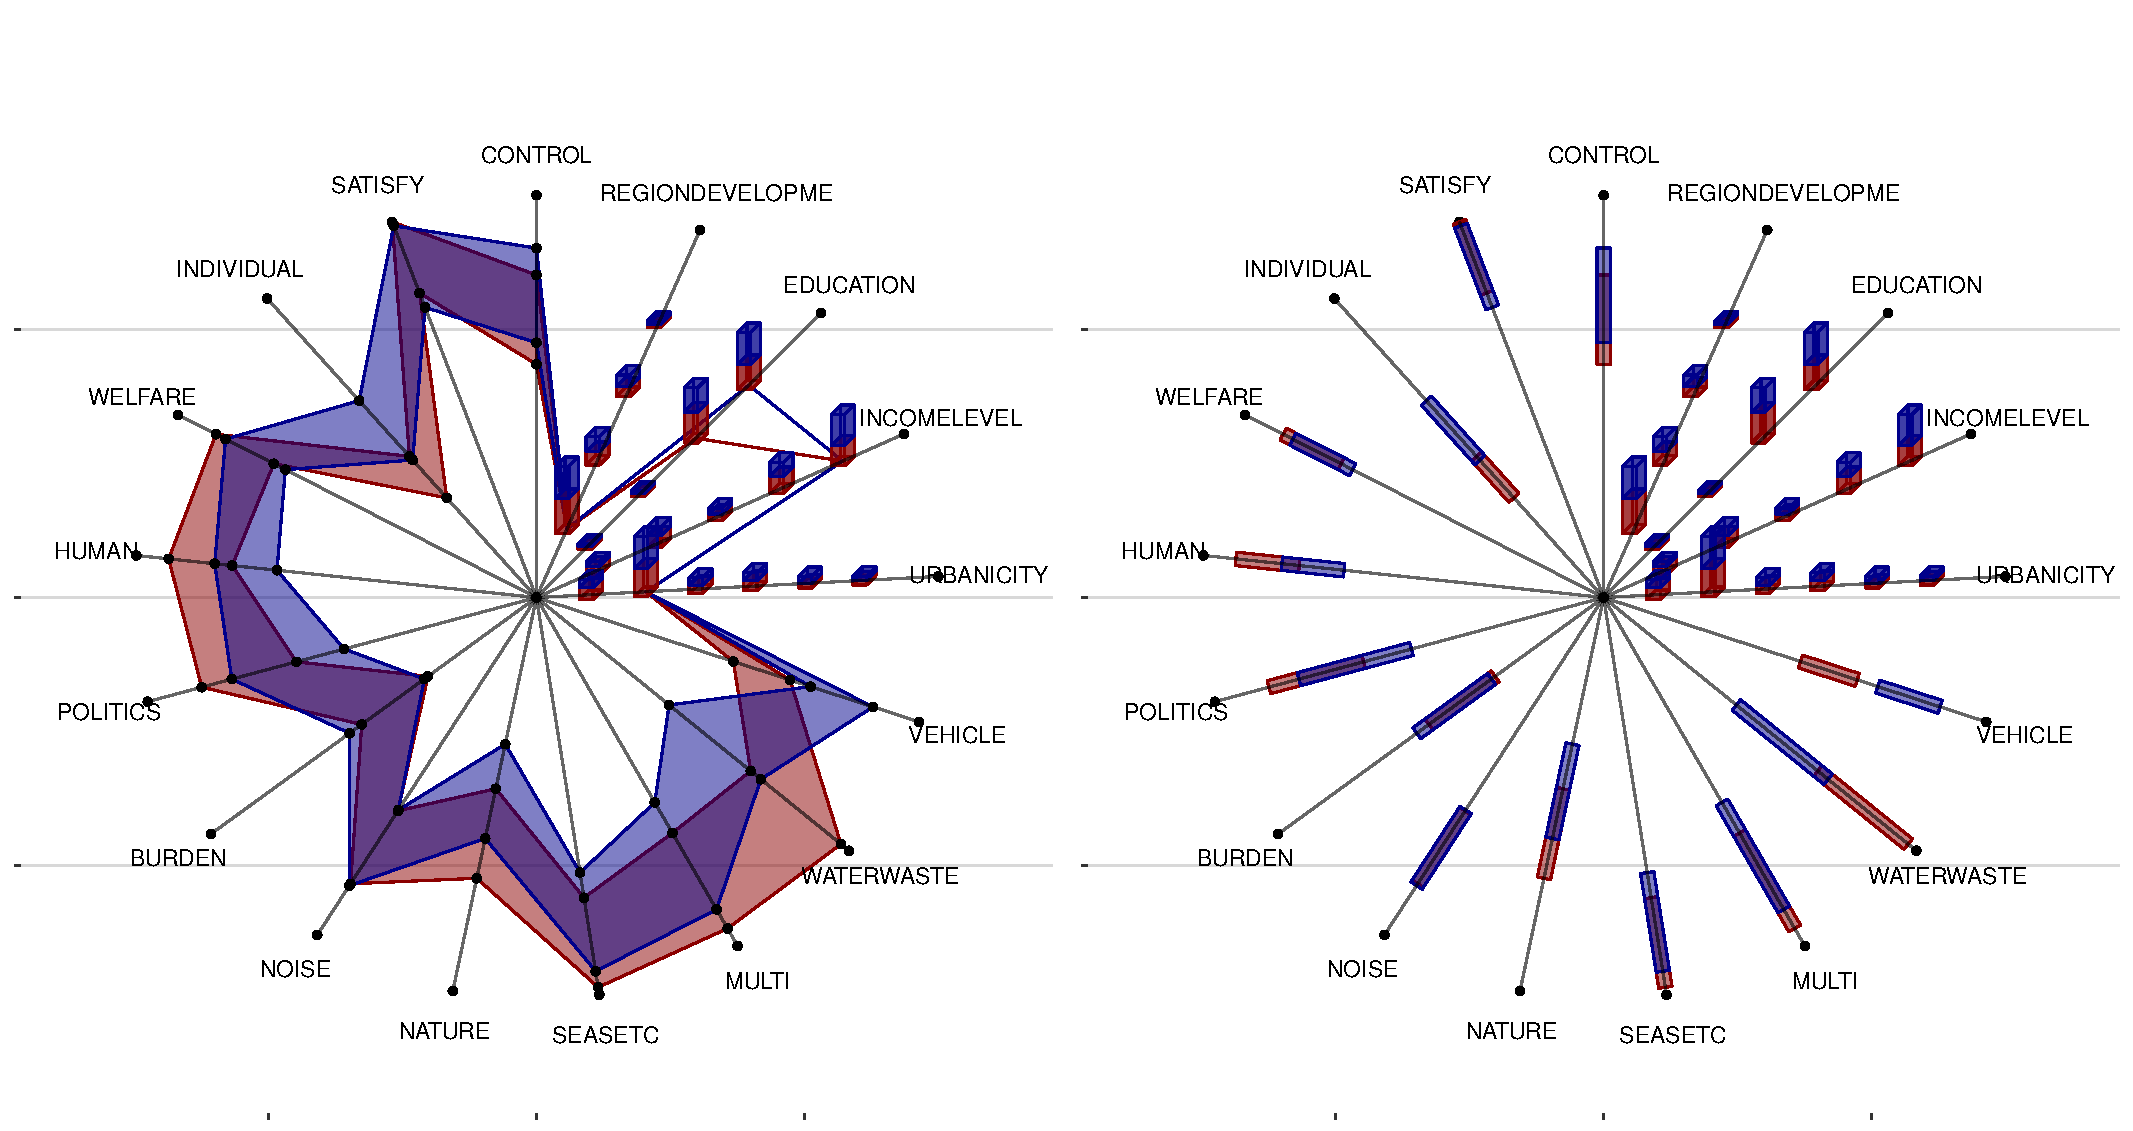
\includegraphics[width=0.9\textwidth]{ggESDA_Jiang&Wu_20210915-radar.pdf} 
\caption{\label{fig:radar}  Compare the distinct observations in the same figure by color mapping.}
\end{figure}

Last but not least, we propose a graphic method based on quantiles. The benefit of this proposed method is that distributional details are visible for the graph. Under the option \code{type = "quantile"}, for example, we divide the quantile percentage of $25\%$ to $75\%$ into the equal subintervals represented as grayscale and shown in Figure \ref{fig:quantile2}. The variable WELFARE of the left panel in the figure depicts the rapid increase close to the 3rd quartiles, which implies it exists a left-skewed distribution. In this way, it becomes more straightforward to extend the comparison of variables to datasets.

\begin{figure}[htbp]
\centering
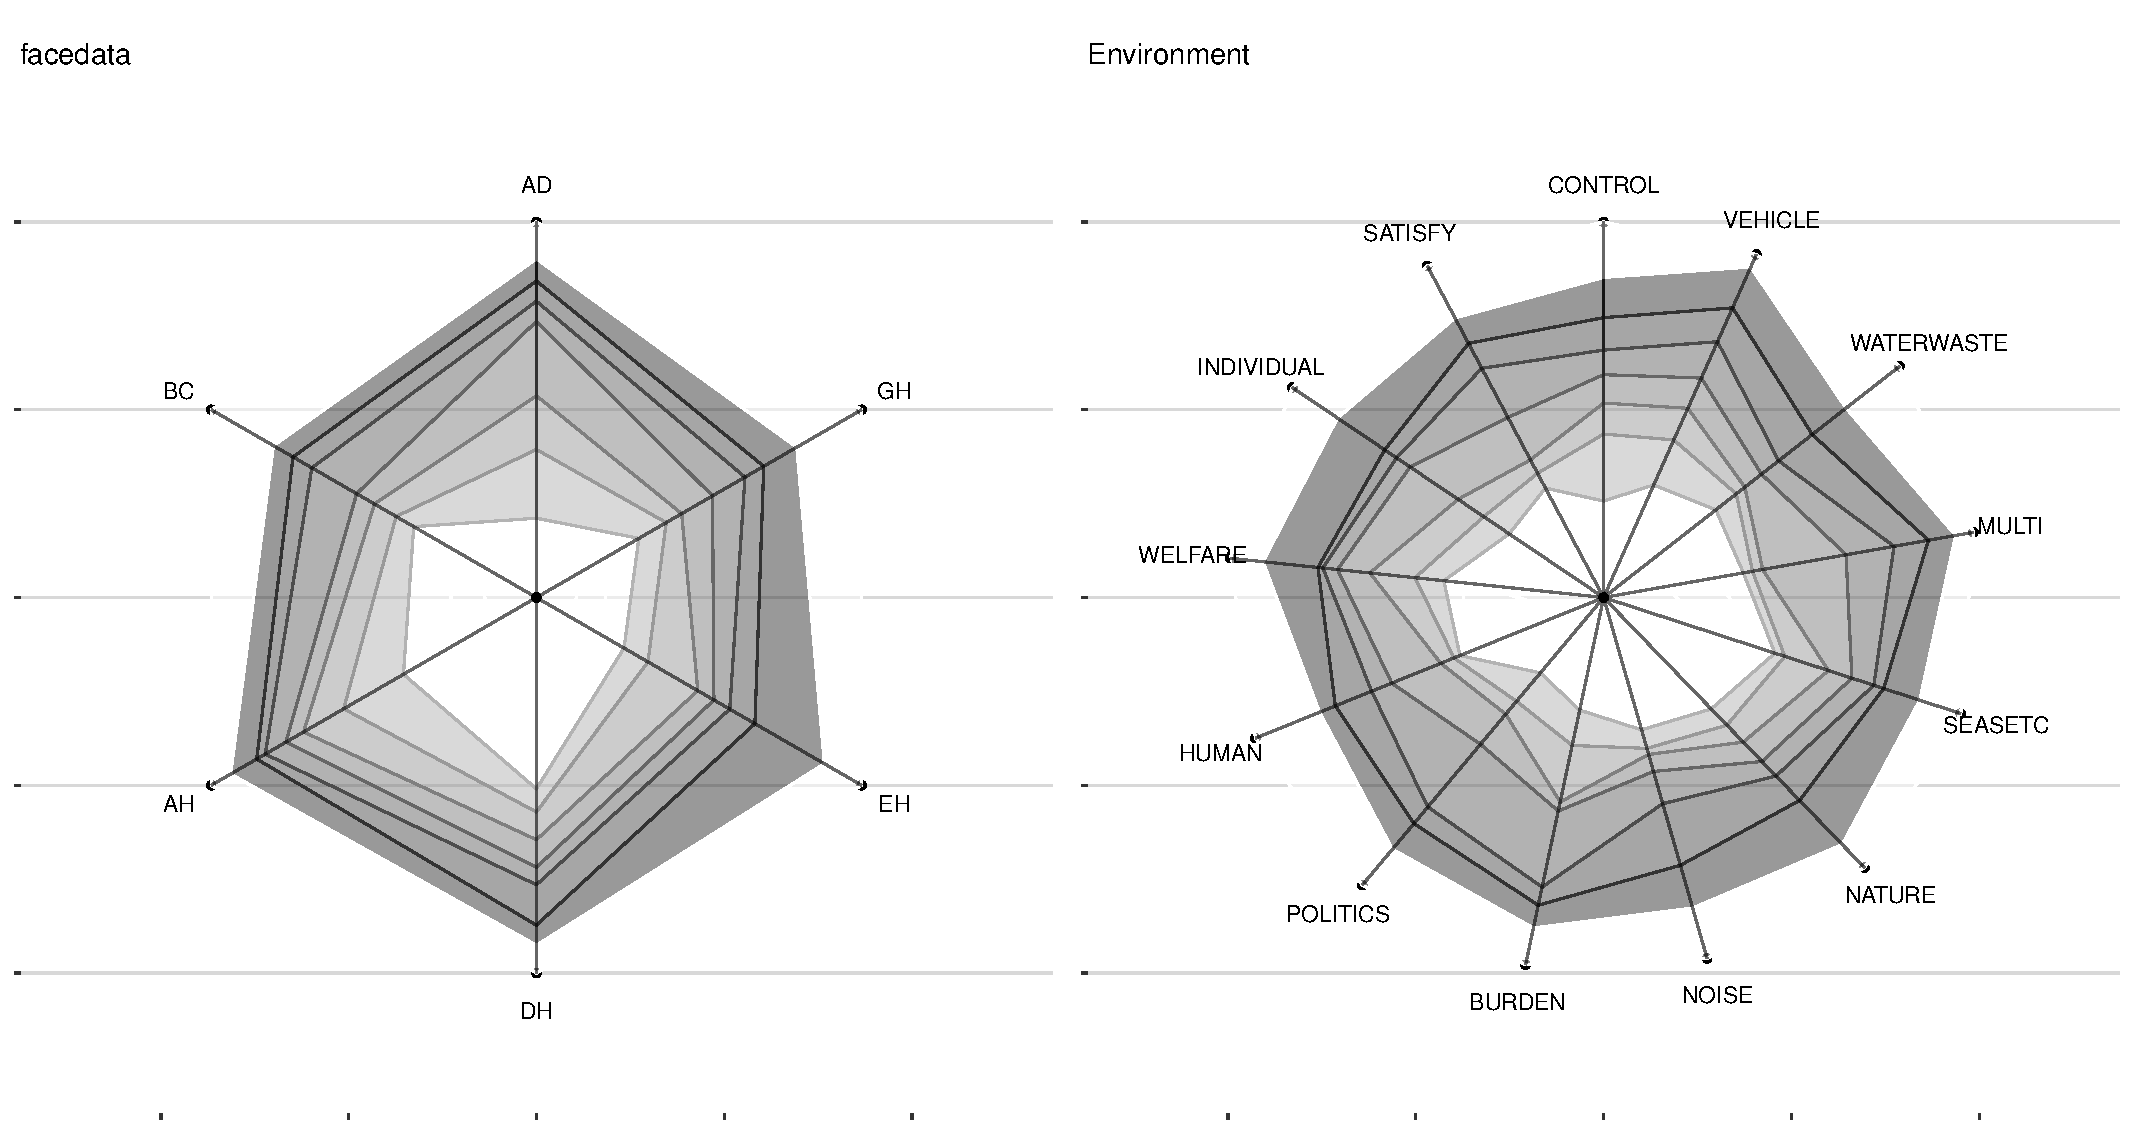
\includegraphics[width=0.9\textwidth]{radar_2datasets.pdf} 
\caption{\label{fig:quantile2} Quantile for two symbolic datasets.}
\end{figure}

%end application

\section{Generalization and Extension}

As far as generalization and extension are concerned, the package provides a simple way for making connections with other useful packages, so that the result of common statistical or machine learning methods on other packages may be visualized as well using \pgk{ggESDA} if it is interval-valued. In addition, we may get the classical data most of the time, so summarization between classical to interval-valued data becomes important. The following will discuss these explicitly. 

\subsection{Generalization with prominent SDA packages}

For the demonstration, we consider two famous \proglang{R} packages for SDA, \pkg{HistDAWass} \cite{irpino2015} and \pkg{MAINT.Data} \cite{Silva2011}. Both of these make lots of contributions to the statistics of SDA, so we tend to generalize these data into the \pkg{ggESDA} type, which may help us to visualize.

\subsubsection{General principle}\label{sec:genPrin}

Generally, it is not merely the well-known packages in \proglang{R} that can make a plot using it. As long as keeping some principle, it will be easily performed:

\begin{enumerate}
  \item Understand the data structure clearly if it is an object from other packages.
  \item Extract the min data and max data from it or make some necessary transformation.
  \item Classify the data you extract belong.
  \item Reorganized it and use \code{classic2sym} for the final transformation.
  \item Visualize the front result using \pgk{ggESDA}.
\end{enumerate}

Because of the interval-valued data, all SDA packages studying in the same field will store and deal with the min and max data. Hence, the transformation method in section \ref{sec:userDef} plays a important role. With the connection being built, it can be compatible with all other tools in \proglang{R}.

\subsubsection[HistDAWass]{\pkg{HistDAWass}}

We further use the principle to process \code{BLOOD} data in \pkg{HistDAWass}, first. With the method \pkg{HistDAWass} provided, it will be more convenient to get min and max data:

\begin{Schunk}
\begin{Sinput}
> library(HistDAWass)
> # Get min and max data
> BLOOD <- HistDAWass::BLOOD
> blood.min <- get.MatH.stats(BLOOD, stat = "min")
> blood.max <- get.MatH.stats(BLOOD, stat = "max")
> blood <- data.frame(blood.min, blood.max)
> # Reorganized and Build ggESDA obj.
> blood.sym <- classic2sym(blood, groupby = "customize",
+                      minData = blood[, 2:4],
+                      maxData = blood[, 6:8])
> # Make names
> blood.names <- get.MatH.main.info(BLOOD)$varnames
> blood.i <- blood.sym$intervalData
> colnames(blood.i) <- blood.names
> head(as.data.frame(blood.i), 5)
\end{Sinput}
\begin{Soutput}
        Cholesterol      Hemoglobin      Hematocrit
1  [80.00 : 240.00] [12.00 : 15.00] [35.00 : 47.00]
2  [80.00 : 240.00] [10.50 : 14.00] [31.00 : 44.00]
3  [95.00 : 245.00] [10.50 : 14.00] [31.00 : 43.50]
4 [105.00 : 260.00] [10.50 : 14.00] [31.00 : 42.50]
5 [115.00 : 260.00] [10.80 : 13.60] [31.00 : 42.50]
\end{Soutput}
\end{Schunk}

After getting the necessary data, classifying data belonging is vital for reorganization, which means that differentiating the min data and max data. For instance, \code{minData = blood[, 2:4]} represents the min data are the columns of $2,3,4$ in this case.

\subsubsection[MAINT.Data]{\pkg{MAINT.Data}}

However, it is also a common way to store interval-valued data by median and range. In \pkg{MAINT.Data}, the data will exist in this form. Fortunately, a median-range form is not difficult to deal with. We can do the necessary conversion directly to get the data we expect:

\begin{Schunk}
\begin{Sinput}
> library(MAINT.Data)
> #get data interval-valued data in AbaloneIdt
> AbaloneIdt <- MAINT.Data::AbaloneIdt
> Aba.range <- AbaloneIdt@LogR
> Aba.mid <- AbaloneIdt@MidP
> #make a necessary transformation for build min max data
> Aba <- data.frame(Aba.min = Aba.mid - exp(Aba.range) / 2,
+                   Aba.max = Aba.mid + exp(Aba.range) / 2)
> # Reorganized and Build ggESDA obj.
> Aba.sym<- classic2sym(Aba, groupby = "customize",
+                       minData = Aba[, 1:7],
+                       maxData = Aba[, 8:14])
> # Make names
> colnames(Aba.sym$intervalData) <- AbaloneIdt@VarNames
> Aba.i <- Aba.sym$intervalData %>% 
+   cbind(Aba.obs = AbaloneIdt@ObsNames) %>% 
+   column_to_rownames(var = "Aba.obs")
> head(Aba.i[, 1:4], 5)
\end{Sinput}
\begin{Soutput}
               Length      Diameter        Height  Whole_weight
F-10-12 [0.34 : 0.78] [0.26 : 0.63] [0.06 : 0.23] [0.21 : 2.66]
F-13-15 [0.39 : 0.82] [0.30 : 0.65] [0.10 : 0.25] [0.27 : 2.51]
F-16-18 [0.40 : 0.74] [0.32 : 0.60] [0.10 : 0.24] [0.35 : 2.20]
F-19-21 [0.49 : 0.72] [0.36 : 0.58] [0.12 : 0.21] [0.68 : 2.12]
F-23-24 [0.45 : 0.80] [0.38 : 0.63] [0.14 : 0.22] [0.64 : 2.53]
\end{Soutput}
\end{Schunk}

In brief, following the general principle in section \ref{sec:genPrin} may facilitate the integration, extend utilize of \pkg{ggESDA} and generalize to all SDA studies.

\subsection{Interval-valued Data Summarization}

Another possibility of the data structure would be a classical data, we provide multiple method for dealing with this kind of transformation. The following would discuss the functionality of \code{classic2sym}.

\subsubsection{Classical Datasets}

We will apply the breast mass dataset, which is computed from a digitized image of a fine needle aspirate (FNA), to demonstrate how does a classical dataset transforms into a symbolic dataset. The breast mass dataset describe characteristics of the cell nuclei present in the image. It can be downloaded from the kaggle at \url{https://www.kaggle.com/uciml/breast-cancer-wisconsin-data?select=data.csv}. There are 569 observations and 32 variables in the dataset. We are going to store this dataset in \code{breastData} as data frame type in \proglang{R}, and the variables will be shown as follows:
\begin{Schunk}
\begin{Sinput}
> colnames(breastData)
\end{Sinput}
\begin{Soutput}
 [1] "id"                      "diagnosis"              
 [3] "radius_mean"             "texture_mean"           
 [5] "perimeter_mean"          "area_mean"              
 [7] "smoothness_mean"         "compactness_mean"       
 [9] "concavity_mean"          "concave points_mean"    
[11] "symmetry_mean"           "fractal_dimension_mean" 
[13] "radius_se"               "texture_se"             
[15] "perimeter_se"            "area_se"                
[17] "smoothness_se"           "compactness_se"         
[19] "concavity_se"            "concave points_se"      
[21] "symmetry_se"             "fractal_dimension_se"   
[23] "radius_worst"            "texture_worst"          
[25] "perimeter_worst"         "area_worst"             
[27] "smoothness_worst"        "compactness_worst"      
[29] "concavity_worst"         "concave points_worst"   
[31] "symmetry_worst"          "fractal_dimension_worst"
\end{Soutput}
\end{Schunk}

Except for the first two variables, they are all composed of mean, standard error, and "worst" in their own field respectively.

\subsubsection{K-means}

K-means clustering is a method of vector quantization, originally from signal processing, that aims to partition n observations into k clusters in which each observation belongs to the cluster with the nearest mean. In \pkg{ggESDA}, the algorithm will be based on the \pkg{stats} package, and the number of k is a parameter that user can define themself:

\begin{Schunk}
\begin{Sinput}
> breastData <- dplyr::select(breastData, -id)
> breastData.sym <- classic2sym(breastData, groupby = "kmeans", k = 5)
> breastData.sym.i <- breastData.sym$intervalData
> as.data.frame(head(breastData.sym.i[, 1:4], 5))
\end{Sinput}
\begin{Soutput}
      diagnosis     radius_mean    texture_mean    perimeter_mean
1 B:0.68 M:0.32 [11.84 : 16.30] [10.89 : 30.72]  [77.93 : 109.80]
2 B:0.04 M:0.96 [13.81 : 19.59] [11.89 : 39.28]  [91.56 : 132.40]
3 B:0.00 M:1.00 [15.50 : 24.25] [10.38 : 32.47] [102.90 : 166.20]
4 B:0.98 M:0.02  [6.98 : 13.05]  [9.71 : 33.81]   [43.79 : 85.09]
5 B:0.00 M:1.00 [20.73 : 28.11] [17.25 : 31.12] [135.70 : 188.50]
\end{Soutput}
\end{Schunk}

The \code{id} is unused in this case, so we remove it by \pkg{dplyr}. Then using \code{classic2sym} to aggregate \code{breastData}. It will return several result sets include clustering result and interval-valued data, etc. The interval-valued data can be extracted by \code{$intervalData}, and it will be presented by the package of \pkg{RSDA} type.

The \code{groupby} is a parameter that determine what kind of aggregation methods will be used. Whenever the K-means method is applied, the consequent \code{k} will become meaningful, whereas the other situation is not. It is also a default method when users have no input arguments in \code{groupby}.

\subsubsection{Hierarchical}

The second well-known clustering algorithm is called Hierarchical clustering \cite{Cecil:1966}, also called hierarchical cluster analysis or HCA. It can be performed with a distance matrix
calculated by raw data and used to present the distance of each cluster. In basic \proglang{R} package, it is also realized by \pkg{stats}, which the \pkg{ggESDA} is based on for implementing HCA:

\begin{Schunk}
\begin{Sinput}
> breastData.sym <- classic2sym(breastData, groupby = "hclust")
> breastData.sym.i <- breastData.sym$intervalData
\end{Sinput}
\end{Schunk}

Remark that the \code{k} parameter is not meaningful in the case without K-means clustering. In \code{classic2sym}, the keywords of HCA is called \code{hclust}.

\subsubsection{Variables Aggregation}

Using a particular variable to merge different data is a common way for data analysis, too. \pkg{ggESDA} provides such as this concept in \code{classic2sym} to analyze different factors of category variables, and merge the same factor into the symbolic data type:

\begin{Schunk}
\begin{Sinput}
> breastData.sym <- classic2sym(breastData, groupby = "diagnosis")
> breastData.sym.i <- breastData.sym$intervalData
> head(breastData.sym.i[, 1:4], 5)
\end{Sinput}
\begin{Soutput}
      radius_mean    texture_mean   perimeter_mean           area_mean
B  [6.98 : 17.85]  [9.71 : 33.81] [43.79 : 114.60]   [143.50 : 992.10]
M [10.95 : 28.11] [10.38 : 39.28] [71.90 : 188.50] [361.60 : 2,501.00]
\end{Soutput}
\end{Schunk}

In \code{breastData}, the only category variable is \code{diagnosis}, which means the diagnosis of breast tissues (M = malignant, B = benign). We put it as an input argument in \code{groupby} for merging different diagnosis results, and the interval-valued data of result sets will display its factor levels in row names.


\subsubsection{User-defined}\label{sec:userDef}

In general, users may not always use the aggregation methods we provide, thus, besides generating a particular variable for the group, \pkg{ggESDA} facilitates the process through the min data and max data that user-defined.

For the demonstration, we will build both min data and max data using \code{runif}. Generate a uniform random variable to make sure that all min data are smaller than max data:

\begin{Schunk}
\begin{Sinput}
> minData <- runif(100, -100, -50)
> maxData <- runif(100, 50, 100)
> demoData <- data.frame(min = minData, max = maxData)
> demoData.sym <- classic2sym(demoData, groupby = "customize", 
+                             minData = demoData$min,
+                             maxData = demoData$max)
> demoData.sym.i <- demoData.sym$intervalData
> as.data.frame(head(demoData.sym.i, 5))
\end{Sinput}
\begin{Soutput}
                V1
1 [-96.02 : 75.19]
2 [-90.44 : 62.66]
3 [-91.34 : 57.60]
4 [-99.93 : 95.67]
5 [-50.04 : 68.89]
\end{Soutput}
\end{Schunk}

Then choose the \code{customize} argument in \code{groupby}, input which data are \code{minData} or \code{maxData}, and the transformation will be simply completed.

In order to simplify the process and make the preprocessing friendly, we develop these methods and let the people who want to analyze symbolic data easier. Overall, the conversion and essential concepts can be summarized in table \ref{tab:classic2sym}. 

% begin table classic2sym
\begin{table}[htbp]
  \centering
  \caption{Summary for \code{classic2sym} function}
  \setlength{\extrarowheight}{6pt}
  \resizebox{\textwidth}{!}{
    \begin{tabular}{cccccc}
    \toprule
    
    \multicolumn{6}{c}{\textbf{\code{classic2sym}}} \\
    \midrule
    \code{groupby} Args. & Transformation & Data Type & Moment & Cluster Result & Require Other Args.  \\
    \midrule
    \code{kmeans} & K-means & Numeric/Category & Smaller data & V     & TRUE \\
    \code{hclust} & Hierarchical & Numeric/Category & Smaller data & V     & FALSE \\
    variable name & Variables aggregation & Numeric/Category & Own the pre-clustering group & -      & FALSE \\
    \code{customize} & User-defined & Numeric & Connect with other packages &  -     & TRUE \\
    \bottomrule
    \end{tabular}}%
  \label{tab:classic2sym}%
\end{table}%
% end table classic2sym

%end classic2sym intro

%end generalize

\section{Conclusion and Future Work}










\bibliography{refs}

\end{document}
